\thispagestyle{plain}
\section{Resolving organoid brain region identities by mapping single-cell genomic data to reference atlases}
\markboth{Resolving organoid brain region identities by mapping single-cell genomic data to reference atlases}{}

\vspace{0.5cm}

Chapter 2 is an adapted version of the article 'Resolving organoid brain region identities by mapping single-cell genomic data to reference atlases' published in \textit{Cell Stem Cell} (2021). I contributed the development of the VoxHunt R package as well as all computational analyses presented in the article.

\vspace{1cm}

\noindent
{\large\textsc{Authors}}

\noindent
Jonas Simon Fleck\textsuperscript{1$*$}, 
Fátima Sanchís-Calleja\textsuperscript{1$*$}, 
Zhisong He\textsuperscript{1}, 
Malgorzata Santel\textsuperscript{1}, 
Michael James Boyle\textsuperscript{2}, 
J. Gray Camp\textsuperscript{3,4,5\$}, 
Barbara Treutlein\textsuperscript{1\$}

\vspace{0.5cm}

\noindent
$\ast$ Equal contribution\\
\$ Corresponding author

\vspace{1cm}

\noindent
{\large\textsc{Affiliations}}

\noindent
\textsuperscript{1} Department of Biosystems Science and Engineering, ETH Zürich, Basel, Switzerland\\
\textsuperscript{2} Max Planck Institute for Evolutionary Anthropology, Leipzig, Germany\\
\textsuperscript{3} Institute of Molecular and Clinical Ophthalmology, Basel, Switzerland\\
\textsuperscript{4} University of Basel, Basel, Switzerland\\
\textsuperscript{5} Current affiliation: Roche Institute for Translational Bioengineering (ITB), Roche Pharma Research and Early Development, Roche Innovation Center Basel, Switzerland

\vspace{1cm}

\noindent
{\large\textsc{Correspondence}} 

\noindent
J. Gray Camp (\href{mailto:grayson.camp@iob.ch}{grayson.camp@iob.ch})\\
Barbara Treutlein (\href{mailto:barbara.treutlein@bsse.ethz.ch}{barbara.treutlein@bsse.ethz.ch})
\vspace{1cm}

\noindent
{\large\textsc{Author contributions}}

\noindent
J.S.F. developed the computational tool and performed computational analyses with support from Z.H. and M.J.B.. F.S.C. designed and executed the patterning experiment with assistance from M.S.. J.S.F., F.S.C., B.T., and J.G.C. designed the study and wrote the manuscript.

\vspace{1cm}

\noindent
{\large\textsc{Article link}} 

\noindent
\href{https://doi.org/10.1016/j.stem.2021.02.015}{https://doi.org/10.1016/j.stem.2021.02.015}


\subsection{Abstract}

Self-organizing tissues resembling brain structures generated from human stem cells offer exciting possibilities to study human brain development, disease, and evolution. These three-dimensional models are complex and can contain cells at various stages of differentiation from different brain regions. Single-cell genomic methods provide powerful approaches to explore cell composition, differentiation trajectories and genetic perturbations in brain organoid systems. However, it remains a major challenge to understand the heterogeneity observed within and between individual organoids. Here, we have developed a set of computational tools (VoxHunt) to assess brain organoid patterning, developmental state, and cell identity through comparisons to spatial and single-cell transcriptome reference datasets. We use VoxHunt to characterize and visualize cell compositions using single-cell and bulk genomic data from multiple organoid protocols modeling different brain structures. VoxHunt will be useful to assess organoid engineering protocols and to annotate cell fates that emerge in organoids during genetic and environmental perturbation experiments.


\subsection{Introduction}

Self-organizing tissues resembling brain structures generated from human stem cells offer exciting possibilities to study human brain development, disease, and evolution. These three-dimensional models are complex and can contain cells at various stages of differentiation from different brain regions. Single-cell genomic methods provide powerful approaches to explore cell composition, differentiation trajectories and genetic perturbations in brain organoid systems. However, it remains a major challenge to understand the heterogeneity observed within and between individual organoids. Here, we have developed a set of computational tools (VoxHunt) to assess brain organoid patterning, developmental state, and cell identity through comparisons to spatial and single-cell transcriptome reference datasets. We use VoxHunt to characterize and visualize cell compositions using single-cell and bulk genomic data from multiple organoid protocols modeling different brain structures. VoxHunt will be useful to assess organoid engineering protocols and to annotate cell fates that emerge in organoids during genetic and environmental perturbation experiments.

Spatiotemporal patterning events occurring during brain development lead to the formation of multiple forebrain, midbrain, and hindbrain structures composed of a diversity of cell types. Portions of this structural and cellular diversity can be recapitulated in stem cell-derived neuronal tissues that self-organize in three-dimensional culture in vitro (\cite{lancaster_generation_2014}). Over the past few years, the generation of human brain organoids and spheroids has enabled unprecedented analyses of human brain development and disease (reviewed in \cite{arlotta_organoids_2018,giandomenico_probing_2017,pasca_rise_2018}), as well as evolution (\cite{kanton_organoid_2019,mora-bermudez_differences_2016,pollen_establishing_2019}). 
There are two general strategies for producing 3D human brain tissue cultures. In the first strategy, pluripotent stem cells are guided to form a layer of neuroepithelial stem cells that can differentiate into neurons. Culturing the neuroepithelium in permissive media can result in the generation of multiple brain structures within the same organoid. This self-patterning strategy (\cite{kadoshima_self-organization_2013,lancaster_cerebral_2013}) offers the potential to understand how different parts of the brain self-organize and interact. However, there are often substantial differences in cell type composition between individual organoids, and between batches grown separately. The alternative strategy is to use signaling molecules or other directive cues to control patterning of the neuroepithelium so that a defined structure forms, such as the cortex (\cite{eiraku_self-organized_2008,kadoshima_self-organization_2013,birey_assembly_2017}), ventral telencephalon (\cite{bagley_fused_2017,birey_assembly_2017,xiang_fusion_2017}), hypothalamus (\cite{qian_brain-region-specific_2016}), thalamus (\cite{xiang_hesc-derived_2019}) and others. Multiple protocols have been published to generate modular brain structures and to create higher-level interactions by fusing two or more brain structures to study neuronal migration or to enable formation of inter-region neuronal connections (\cite{bagley_fused_2017,birey_assembly_2017,duan_model-based_2019,pasca_rise_2018}). This technique might increase reproducibility of structure formation, but researchers have yet to define all of the signals that create each brain structure. Moreover, it is unclear whether certain parts of the brain can form in the absence of adjacent structures. 

Despite incredible progress in human brain organoid engineering, it is not yet possible to create a stereotypic organoid containing multiple brain structures.
Organoid protocol development requires robust strategies to assess organoid composition. Single-cell mRNA sequencing (scRNA-seq) has emerged as a high-resolution approach to deconstruct organoid cell composition and reconstruct differentiation trajectories in these complex developing tissues (\cite{camp_human_2015,kanton_organoid_2019,quadrato_cell_2017,velasco_individual_2019}). Multiple labs have used scRNA-seq to assess heterogeneity in brain organoids, and direct comparison between engineered in vitro cortical structures and primary in vivo counterparts have revealed remarkable similarity in gene expression profiles (\cite{camp_human_2015,pollen_establishing_2019}). However, it still remains a major challenge to understand and interpret gene expression and regulatory patterns from organoid single-cell genomic data. 

Here, we have developed a computational toolbox to assess brain organoid patterning, developmental state, and cell identity through systematic comparisons to annotated reference datasets (Figure 2.1). Primarily, we utilize in situ hybridization data from the Developing Mouse Allen Brain Atlas (ABA) as a well-annotated spatial gene expression map. Based on their transcriptome or accessible chromatin landscape, cells can be mapped to voxels, in this case 3D positions rendered from spatial transcript patterns, which enables characterization and visualization of organoid regional composition. In addition, we provide an interface to perform comparisons to bulk RNA-seq data from human microdissected brain structures (BrainSpan, \cite{thompson_high-resolution_2014}) as well as to single-cell RNA-seq data from the developing mouse brain (\cite{la_manno_molecular_2021}). Finally, we show that VoxHunt can help deconvolute bulk organoid transcriptome data as well as assess brain region composition in organoids grown under different conditions. Altogether, VoxHunt will be useful to assess organoid engineering protocols and to rapidly annotate cell fates that emerge in organoids during genetic and environmental perturbation experiments.


\subsection{Results}


\topparagraph{Spatiotemporal voxel maps of the developing mouse brain}
To facilitate exploration of 3D gene expression patterns in the developing brain, we obtained in situ hybridization data of the mouse brain in 8 different developmental stages (Figure 2.2a) from the Allen Developing Mouse Brain Atlas (\cite{thompson_high-resolution_2014}). This dataset is currently the most comprehensive spatially registered four-dimensional reference atlas of a mammalian brain. The dataset provides three-dimensional spatial expression patterns from different experiments that measure a total of 2,073 genes over time points ranging from mouse embryonic day 11.5 through postnatal day 56. Each expression quantification is registered to a single voxel grid for each timepoint (80 - 200 µm resolution) (Figure S2.1a). Each voxel is further annotated with a brain structure derived from a hierarchical structure ontology. We preprocessed this data by summarizing in situ hybridization quantifications from different experiments measuring the same gene to obtain a single gene expression vector for each voxel at each developmental stage. To allow for comparison of structures with similar size throughout developmental stages, we further introduced additional layers of structure annotation by aggregating existing ontological levels, resulting in spatially and temporally resolved brain structures (Figure 2.2b, Figure S2.1b).

\begin{figure}[t!]
    \centering
	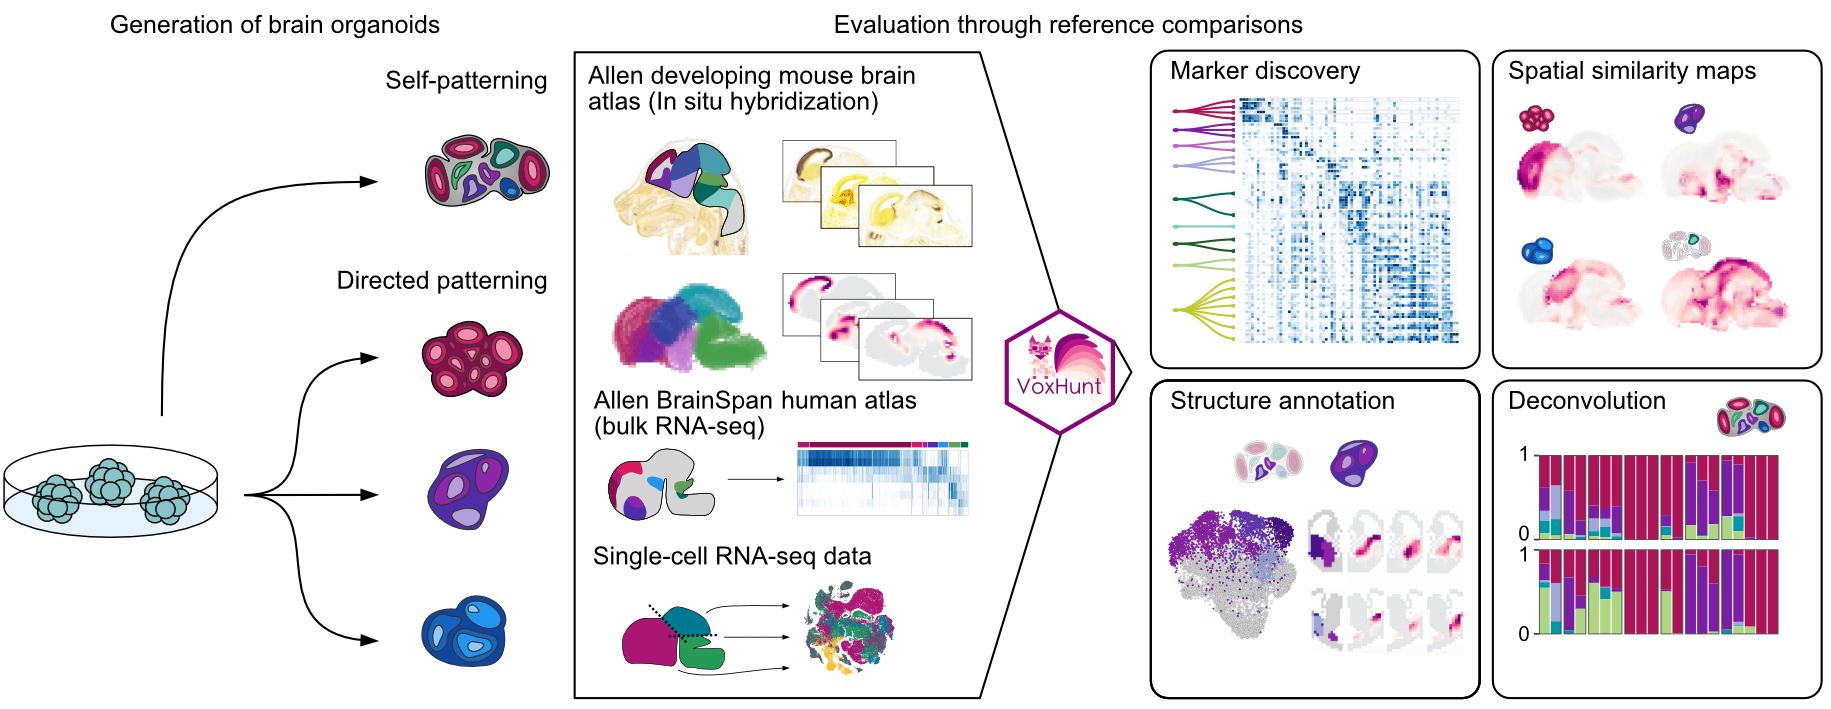
\includegraphics[width=\textwidth]{figures/voxhunt/Figure_1}
    \caption{\textbf{Overview of the VoxHunt computational toolkit for exploring heterogeneity in the developing brain and brain organoid counterparts.}
    Brain organoids generated through various protocols or patterning regimens can give rise to cells resembling different brain structures. VoxHunt helps interpret transcriptomic or epigenomic data from these organoids by providing an interface to relevant reference datasets. VoxHunt implements functions to extract brain structure markers, compute similarity maps of organoid cells, assign regional identities, and deconvolute bulk RNA-seq data into structure proportions.}
    \label{fig:vox1}
\end{figure}



\begin{figure}[t!]
    \centering
	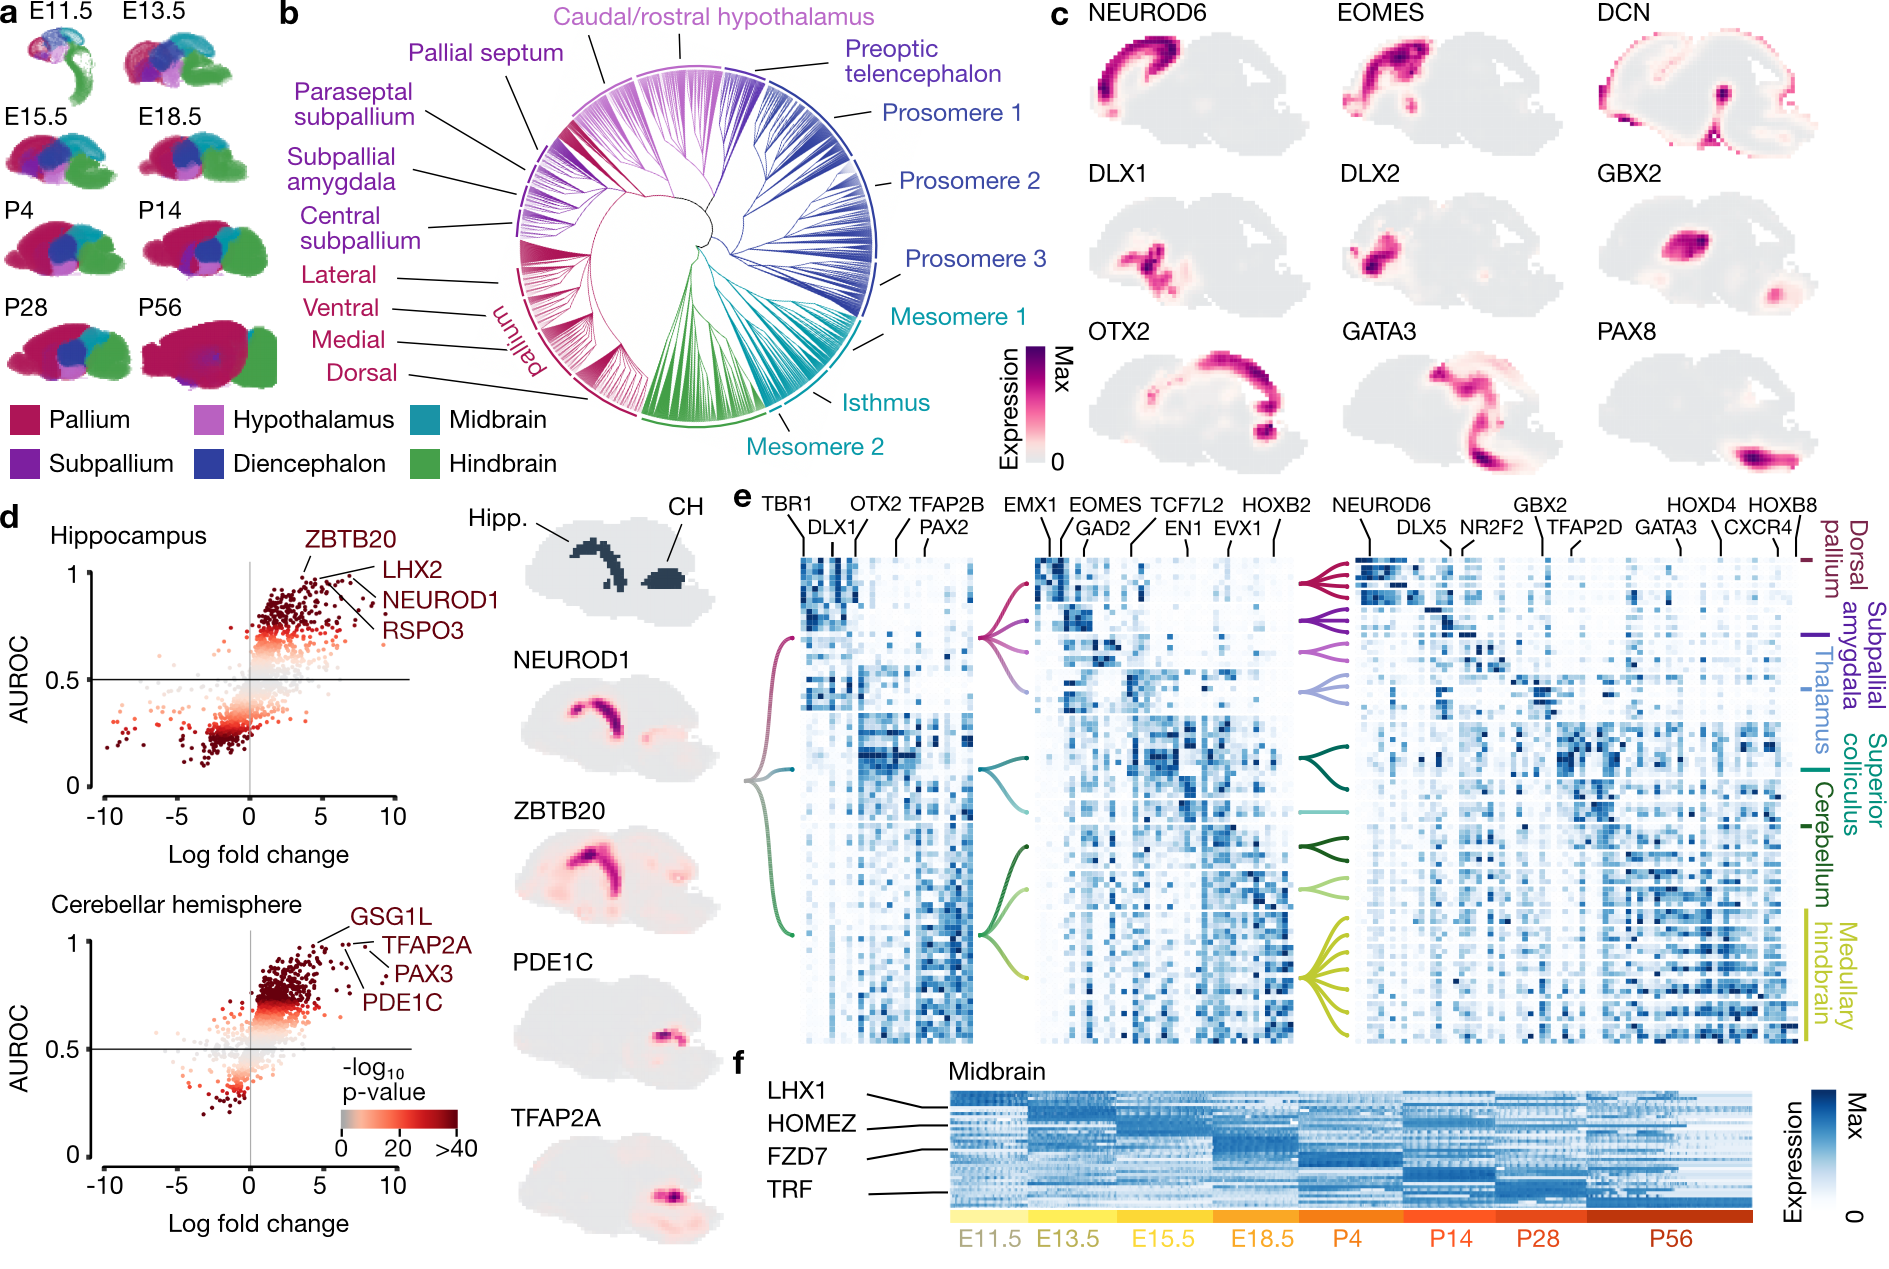
\includegraphics[width=\textwidth]{figures/voxhunt/Figure_2}
    \caption{\textbf{Feature extraction from voxel maps of developing mouse brain in situ hybridization data.} (A) Schematics show mouse brain development over time, with high-level structure annotations color-coded. (B) Dendrogram showing the hierarchically organized structure ontology from the Allen Developing Mouse Brain Atlas. (C) Spatial expression patterns of selected markers as maximum intensity projections across five central sagittal sections (8–12) in the E15.5 mouse brain. (D) Scatterplot showing feature selection for two brain structures, hippocampus (Hipp.) and cerebellar hemisphere (CH), at E15.5, together with the expression profile for the top two marker genes per structure. (E and F) Heatmap showing marker gene expression across brain structures at different levels of structure resolution at stage E15.5 (E) and across developmental stages for the midbrain (F).}
    \label{fig:vox2}
\end{figure}


\topparagraph{Brain structure marker identification}
We performed differential expression analysis between annotated brain structures and used the single-feature area under the receiver operating characteristic curve (AUROC) as a metric for selecting structure-specific genes with spatially confined expression (Figure 2.2c-d, Figure S2.1c). In this way, one can perform large-scale feature selection based on various criteria such as structure- or stage-specificity (Figure 2.2e-f, Figure S2.1d). These brain structure-enriched gene expression profiles could serve as a resource of marker genes to validate cell fate engineering and organoid protocols.



\topparagraph{VoxHunt accurately maps reference populations}
We first validated that the mouse ISH reference atlas is a suitable resource for cell annotation of human single-cell transcriptome data. We used VoxHunt to map single-cell transcriptome data (split-pool barcoding) from the developing mouse brain (\cite{rosenberg_single-cell_2018}), which resulted in mouse-to-mouse mapping of annotated cell populations to voxelized structures (Figure S2.2a). Using this dataset, we assessed the accuracy (fraction of cells with correctly assigned structures) and contrast (similarity to second best structure/similarity to assigned structure) of the spatial mapping under different conditions for feature selection (e.g. differentially expressed genes between structures vs. most variable features), and tested the stability of structure assignments through downsampling of unique molecular identifier (UMI) in the single-cell RNA-seq data (Figure S2.2b-d). We found that accuracy was proportional to the number of features used, and this result was consistent across brain structures. However, for certain structures (e.g. pallium), contrast decreased at low or high feature inclusion. Accuracy has some dependency on UMI count, with certain structures (e.g. Rostral midbrain) being more sensitive to this aspect of the scRNA-seq data. Nonetheless, even with the relatively sparse split-pool barcoding data, we could identify optimal parameters that facilitated mapping with high accuracy and contrast. We then compared bulk RNA-seq data from microdissected human brain structures from the ABA BrainSpan Developing Human Brain Atlas (\cite{thompson_high-resolution_2014}) (S2b,c), as well as four scRNA-seq datasets from primary human brain tissues (\cite{fan_spatial_2018,nowakowski_spatiotemporal_2017,polioudakis_single-cell_2019,zhong_single-cell_2018}) (Figure S2.3). We found that each of the datasets exhibited consistently clear similarity patterns, supporting the use of mouse 4D gene expression data to match homologous brain regional data and predict properties of human cell types.


\begin{figure}[H]
    \centering
	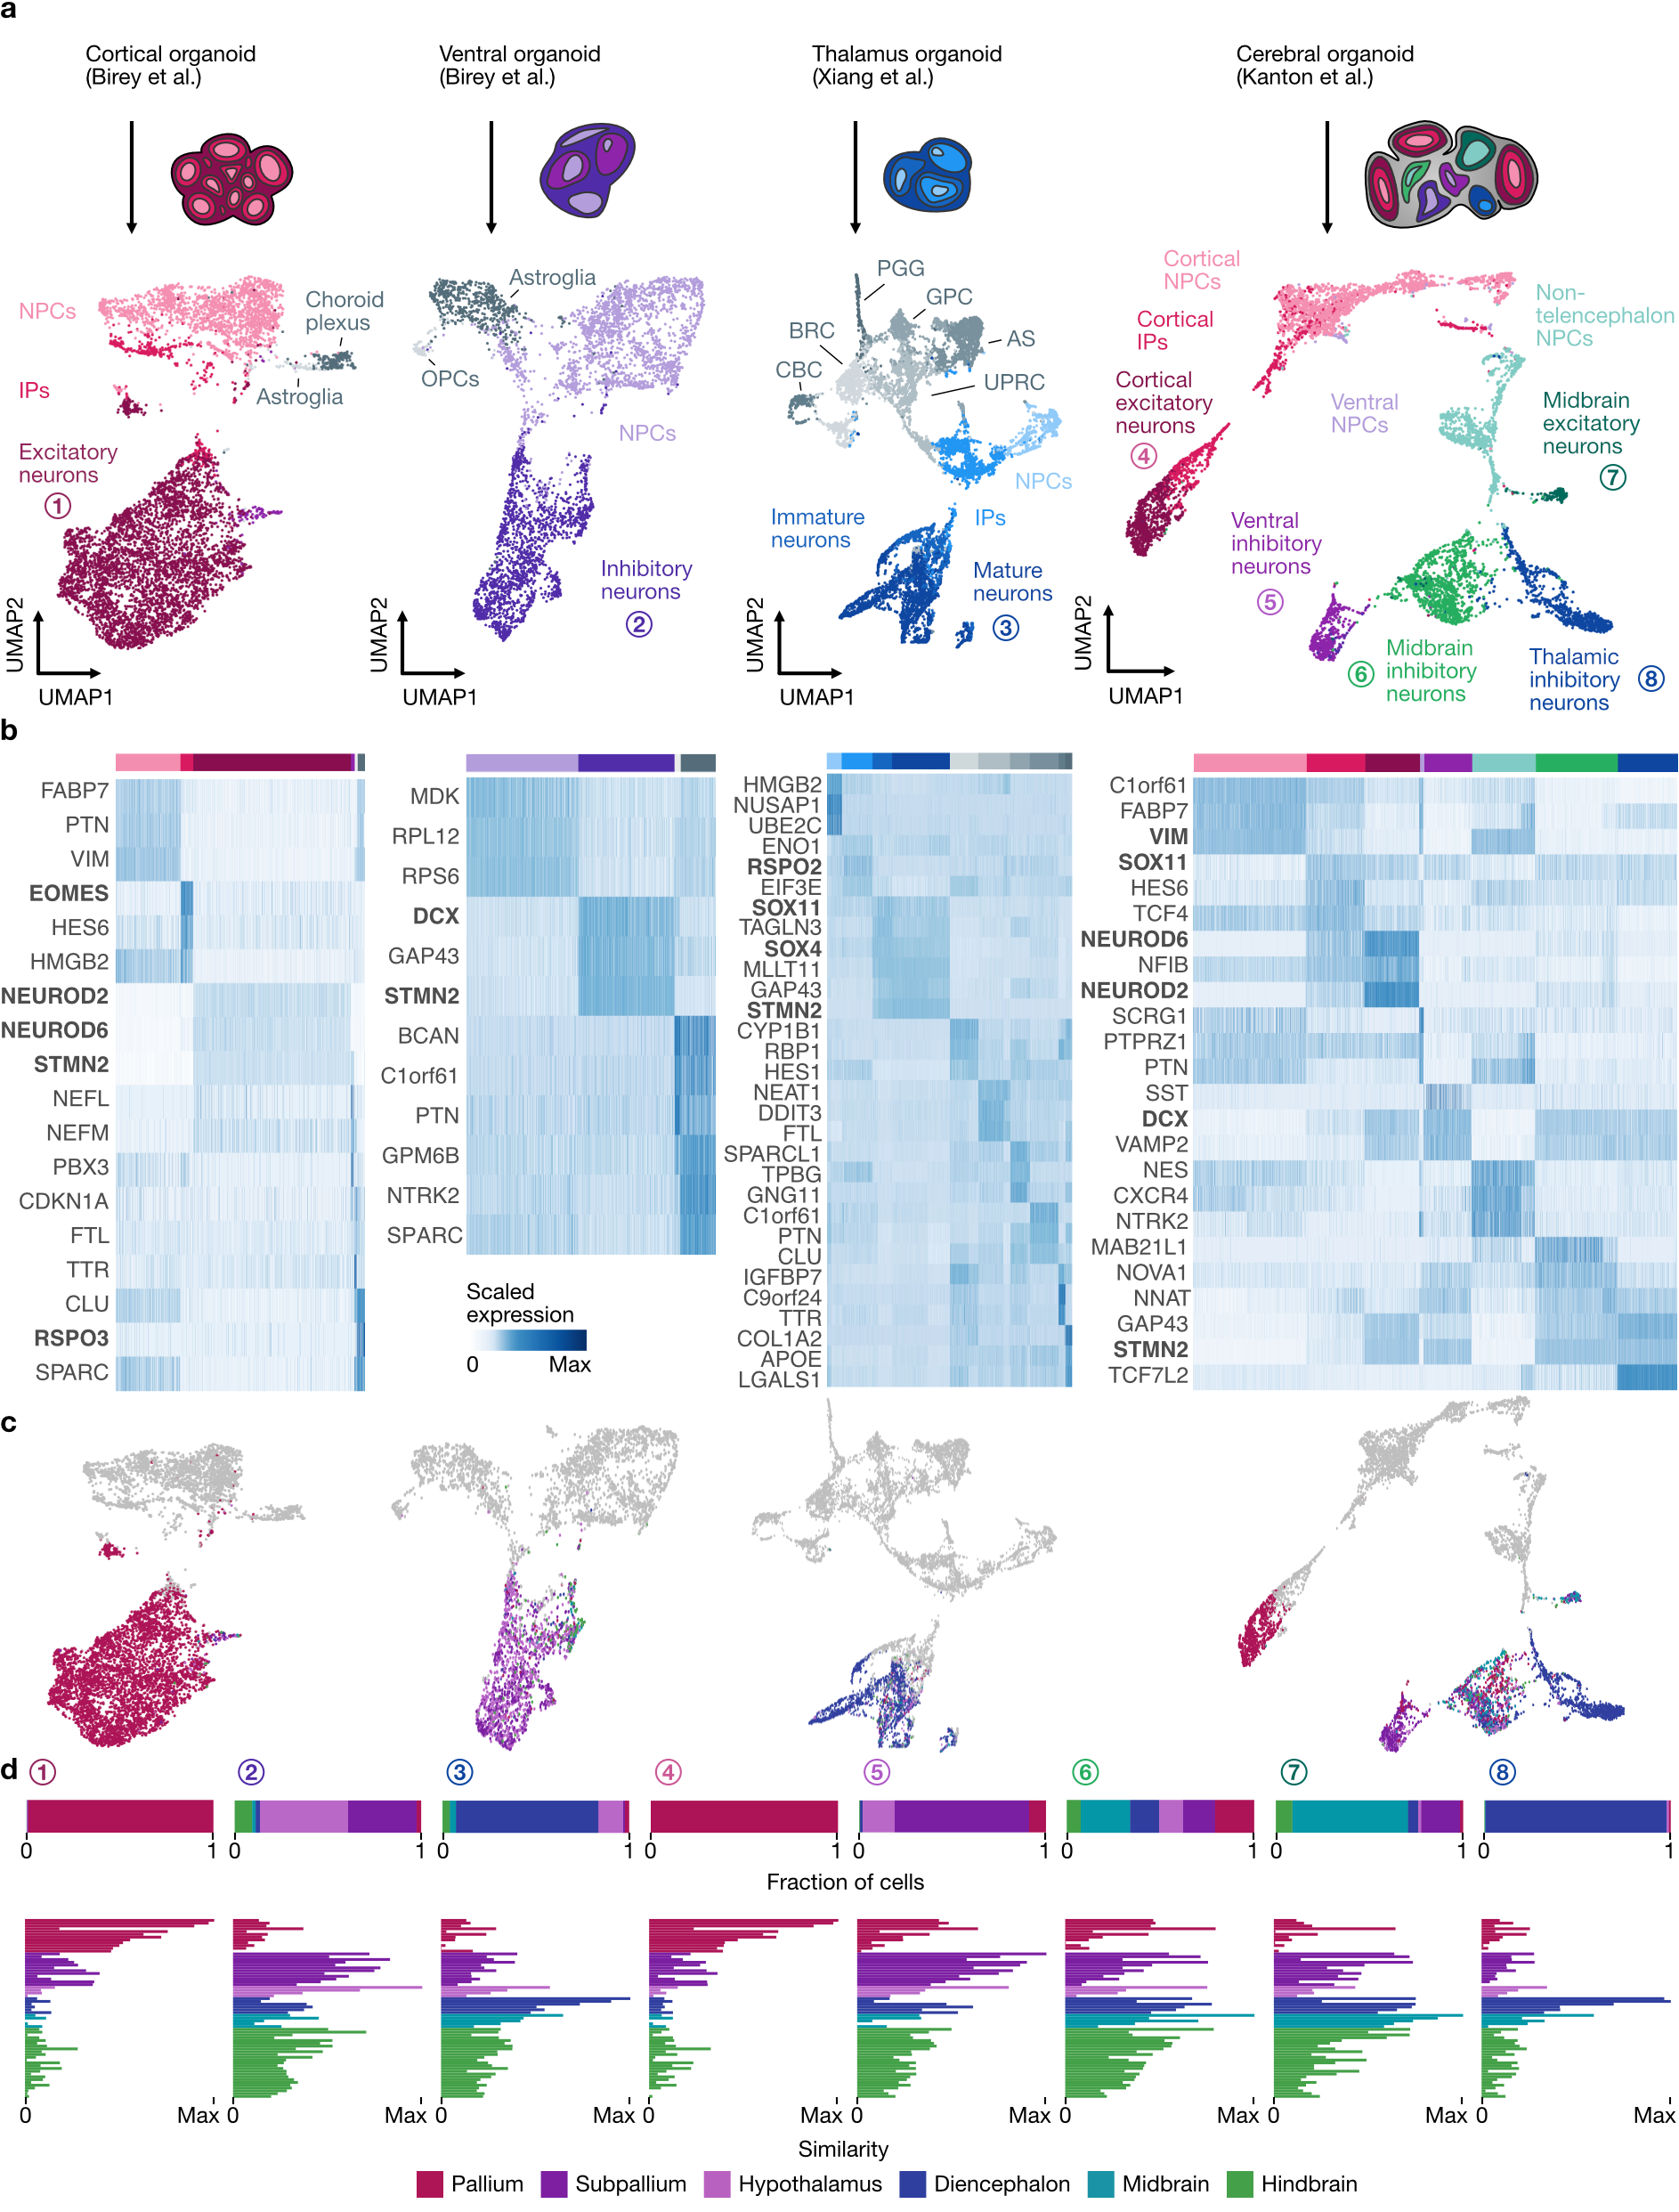
\includegraphics[width=0.9\textwidth]{figures/voxhunt/Figure_3}
    \label{fig:vox3}
% \end{figure}

% \begin{figure}[t!]
%     \centering
    \caption{\textbf{Single-cell transcriptomes deconstruct region composition in brain organoids} (A) UMAP projections of published single-cell transcriptome data from different organoid protocols, including cortical (Birey et al., 2017), ventral (Birey et al., 2017), thalamus (Xiang et al., 2018), and cerebral (Kanton et al., 2019). Cells are colored based on the annotations in the original publications. (B) Heatmap showing the expression of top marker genes for each cluster. Canonical marker genes are highlighted in bold. (C) UMAP projections of neuronal cells from each dataset colored by structure annotation of the voxel with maximum correlation. (D) Top: fraction of cells from each cluster annotated in (A) that have maximum correlation to each brain structure based on comparison to in situ hybridization voxel maps. Bottom: bar plots showing the mean similarity of each cluster to different brain structures. Each bar represents one brain structure at custom annotation level 4.
    IP, immediate progenitor; NPC, neural progenitor cell; OPC, oligodendrocyte progenitor cells; CBC, cilia-bearing cells; BRC, BMP-related cells; PGG, proteoglycan-expressing glia; GPC, glial progenitor cell; AS, astrocytes; UPRC, unfolded protein response-related cells.}
\end{figure}



\topparagraph{Organoid region composition annotation}
We next tested if VoxHunt could be used for unsupervised annotation of cell types generated through different organoid protocols. For this, we obtained published single-cell transcriptome data from three brain structure-specific organoid protocols (thalamus, cortex, ventral telencephalon) (\cite{birey_assembly_2017,xiang_hesc-derived_2019}) as well as one cerebral (unpatterned) organoid protocol (\cite{kanton_organoid_2019}). We used Uniform Manifold Approximation and Projection (UMAP) (\cite{becht_dimensionality_2019}) embeddings to project cells onto a two-dimensional space for each protocol, and annotated the clusters as described in the original studies (Figure 2.3a). All four datasets exhibit a diversity of cell populations, including heterogeneous progenitor and neuronal cells. For neuronal cells from structure-specific organoids, successful patterning is supported by the expression of canonical marker genes (Figure 2.3b). For cerebral organoids, multiple brain structures can form in any given organoid, and marker gene expression analysis suggests the emergence of neuronal cell types from the telencephalon (pallium, subpallium), diencephalon, midbrain, and hindbrain supporting the annotations reported in the original publication (Figure 2.3b). We assessed if annotations from each dataset could be confirmed by correlating single-cell transcriptomes from each neuronal cluster with in situ expression patterns in the mammalian brain at high-level annotations that are consistent across time for telencephalon (pallium, subpallium), diencephalon, midbrain, and hindbrain (Figure 2.3c,d). Cells annotated as cortical neurons derived from both cortical or cerebral organoid protocols showed far higher correlation to pallium than to any other structure. Thalamic neurons showed a similarly clear pattern, with the majority (>90\%) of cells having the highest correlation to voxels within the diencephalon. For clusters of inhibitory neurons annotated as ventral telencephalon, we observed differences between the two organoid protocols. While cells derived from cerebral organoids had consistently higher correlation with subpallial structures, a large fraction of cells (48.3\%) from ventrally patterned organoids were most highly correlated with the hypothalamus. Cell clusters annotated as midbrain neurons derived from cerebral organoid protocols showed a noisier correlation pattern and overall lower correlation to in situ maps than any of the other clusters. While average correlation within each cluster was highest to the midbrain, correlation of single cells did not show clear agreement, especially for cluster 6 annotated as ‘midbrain excitatory neurons’.

\begin{figure}[t!]
    \centering
	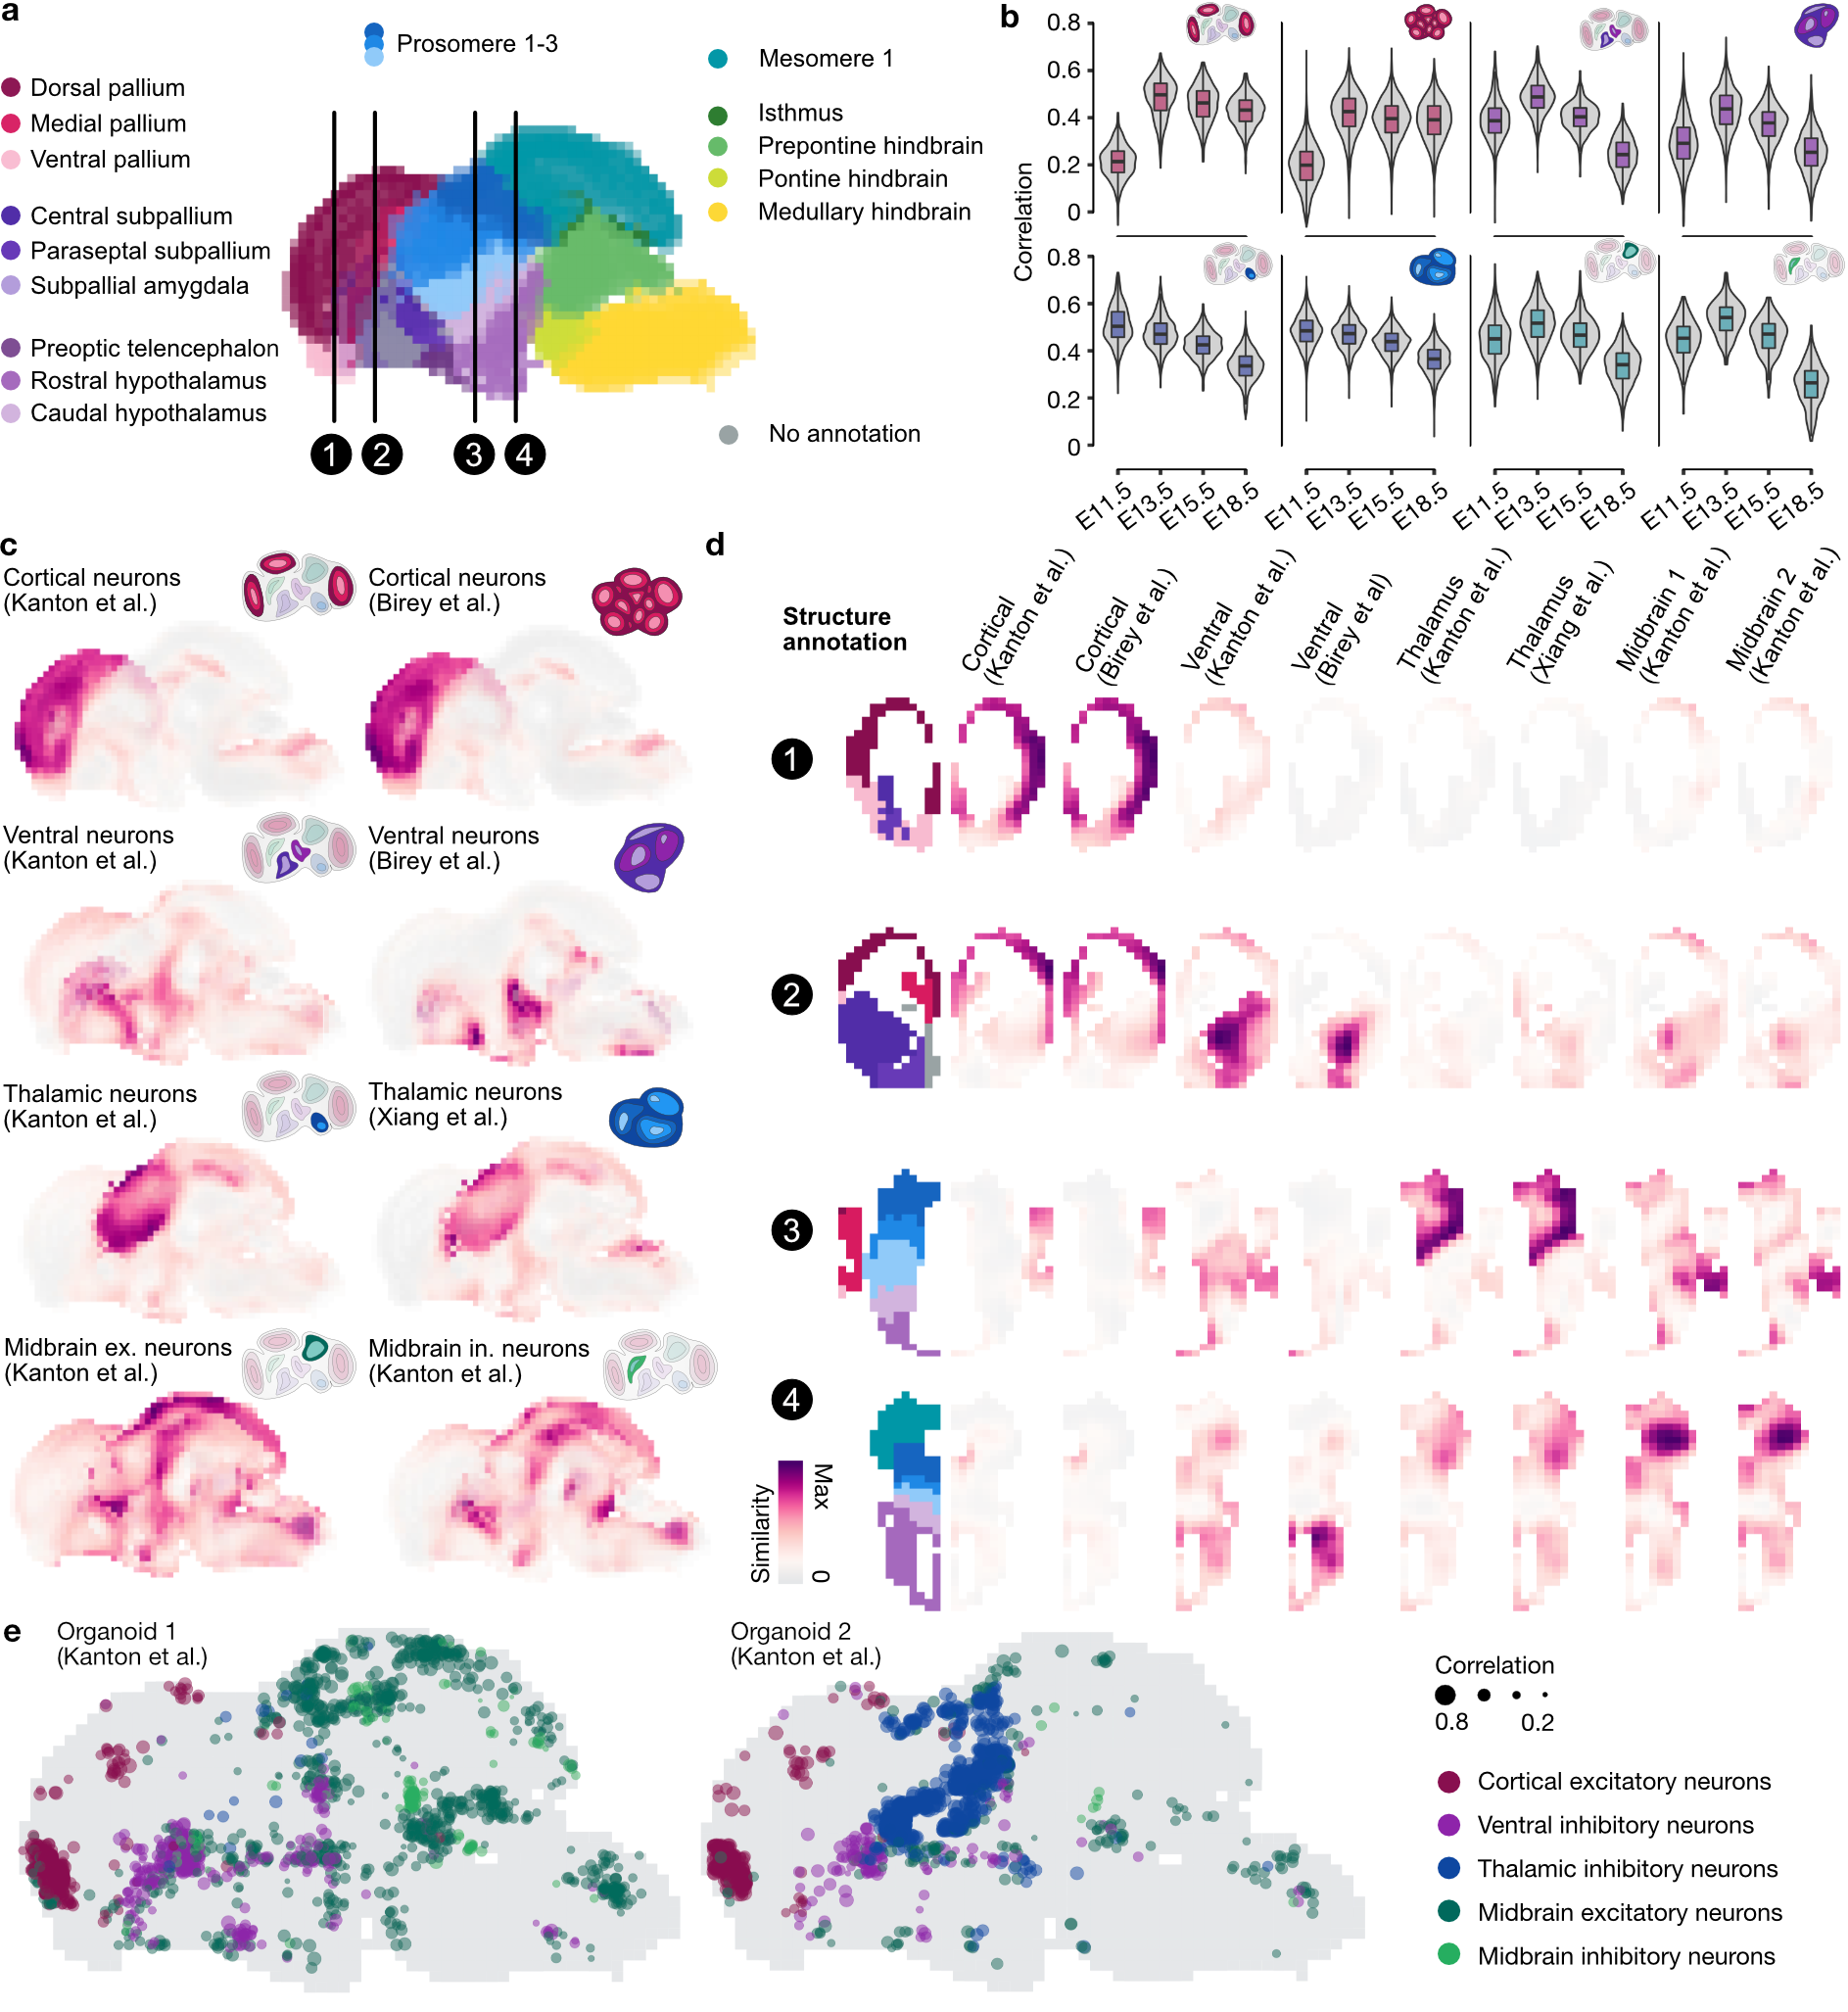
\includegraphics[width=0.9\textwidth]{figures/voxhunt/Figure_4}
    \caption{\textbf{Comparing brain organoid cell populations to spatial brain maps.} (A) Structure annotations of the E13.5 mouse brain (sagittal view), which was used for organoid cluster annotation. Locations 1–4 are used for coronal sections shown in subsequent panels. (B) Violin plots showing the organoid cluster correlation distributions to voxel maps of the previously assigned structure (pallium, subpallium, diencephalon, and mesencephalon) across different developmental time points. (C) Sagittal projections colored by scaled similarity scores of different organoid clusters from each dataset to voxel maps of the E13.5 mouse brain. (D) Coronal sections visualizing regional annotation and scaled similarity scores to different brain structures from different clusters and protocols. (E) Sagittal view of a maximum-correlation projection of cells from two individual cerebral organoids to 8 central sections (5–12) of the E13.5 mouse brain.}
    \label{fig:vox4}
\end{figure}


\topparagraph{Spatial projection of organoid cell transcriptomes}
To select a suitable developmental stage for voxel-resolved visualization of spatial similarity patterns, we computed the correlation of each cell in a cluster to its matching structure from all fetal developmental stages (E11.5 - E18.5) (Figure 2.4a, Figure S2.4a). From the previously decomposed clusters, the majority showed the highest median correlation to E13.5, with the exception of thalamic neuron clusters, which were most highly correlated with structures at E11.5 (Figure 2.4b). For cortical neurons, we further found that their most similar developmental stage was proportional to the age of their organoid of origin (Figure S2.4b,c). For each organoid cluster, we visualized the correlation to each voxel in either a sagittal view (Figure 2.4c, Figure S2.4a) or two-dimensional coronal (Figure 2.4d) sections. To further aid the assessment of cell type compositions of individual organoids, each cell from each organoid can be projected to spatial locations within the brain based on maximum similarity to loci within the voxel maps (Figure 2.4e). These analyses reveal the spatial location within the brain tissue where each cluster or cell has maximal correlation, which can be used to assess the specificity of the regional neuronal population and help annotate previously unknown cell populations. Similarity patterns can also be explored in three-dimensional registrations of the voxel maps (Supplementary Videos 2.1-2.5). 

\topparagraph{Complementary reference datasets as high-dimensional search spaces}
To test whether the structure annotations obtained from mapping to ISH data could be further enhanced through other reference datasets, we compared organoid-derived neurons to time course bulk RNA-seq data from the human brain (BrainSpan) (\cite{thompson_high-resolution_2014}) (Figure S2.4d) as well as a single-cell transcriptomic atlas of the developing mouse brain (\cite{la_manno_molecular_2021}) (Figure S2.4e). Similarities of neuronal clusters to BrainSpan samples largely agreed with the comparison to ISH data. However, BrainSpan covers a limited number of brain structures and lacks midbrain samples, which makes it unsuitable for annotating neurons from certain protocols. The single cell atlas of the developing mouse brain provides coarse (forebrain, midbrain, hindbrain; Figure S2.4e) annotations of cell types arising during early mammalian brain development, and provides functional annotations which cannot be derived from the ISH data alone. We found that organoid-derived cortical neurons showed the highest similarity to excitatory neurons, while ventral neurons mapped to inhibitory (GABA-ergic) neurons, which is in line with expectations (Figure S2.4f). Comprehensive whole brain scRNA-seq datasets from human and mouse will be valuable references for functionally annotating neuronal and non-neuronal cell types.

\topparagraph{Assessing region specificity across organoid protocols}
We used VoxHunt to assess cell identities generated in organoids from different protocols. We analyzed scRNA-seq data from 9 different organoid protocols (\cite{bhaduri_cell_2020,birey_assembly_2017,giandomenico_cerebral_2019,kanton_organoid_2019,pellegrini_human_2020,pollen_establishing_2019,velasco_individual_2019,xiang_hesc-derived_2019}) that have been reported to generate diverse neuronal populations. We found that spatial similarity maps and assigned region identities by VoxHunt corresponded well with the original annotations (Figure S2.5). We found that choroid plexus (ChP) cells from central nervous system barrier forming organoids (\cite{pellegrini_human_2020}) showed a distinct correlation to the roof plate of the invaginated telencephalic vesicle, a ChP precursor. In some cases, VoxHunt enabled annotation of neuronal cell populations with a previously uncertain identity. For example, we observed that neurons in ChP organoids mapped distinctly to diencephalon structures, and appear distinct from neurons generated through a telencephalic organoid protocol (Figure S2.5i). We also observed substantial brain region composition heterogeneity between individual cerebral organoids consistent with previous reports (\cite{kanton_organoid_2019}), especially when comparing organoids from different human iPSC lines (Figure S2.5j). In comparison, the majority of cells from the dorsal forebrain organoid model match pallial structures across organoids and iPSC lines. We note that we were able to annotate a previously unknown cluster present in 1 month old cerebral organoids (\cite{camp_human_2015}) (Figure S2.6a,b). This population was marked by RSPO2/3 and WNT2B which localizes to the invaginated telencephalic roof plate (\cite{kamata_r-spondin_2004}) and transient structures annotated as pallium at the boundary of the developing telencephalon and diencephalon (Figure S2.6c-e). 

\topparagraph{Annotating organoid cell identity at substructure resolution}
We were curious if we could go beyond the structure ontology provided by the ABA to reveal a higher-resolved annotation of organoid cell types. For this, we selected two high-level structures, the dorsal pallium and the subpallium and performed unbiased clustering on voxel transcriptomes (Figure 2.5a,b). We aggregated these clusters based on the expression of canonical marker genes to reveal neural progenitor cell (NPC), immediate progenitor (IP) and neuronal layers in the dorsal pallium and the lateral, medial and caudal ganglionic eminences (LGE, MGE, CGE) in the subpallium. These custom annotations matched the correlation patterns of single-cell transcriptomic data derived from the annotated structures in mice (\cite{loo_single-cell_2019,mayer_developmental_2018}) as well as the expected anatomic position and morphology (Figure 2.5c,d). We found that organoid cells from the cortical trajectory clearly mapped onto the annotated pallial zones (Figure 2.5e). Moreover, ventral neuron clusters from cerebral organoids could be clearly annotated as LGE, MGE or CGE-like interneurons based on their similarities to the substructures (Figure 2.5f). We further used these newly annotated subpallial structures to resolve and compare the heterogeneity of inhibitory neurons derived from three organoid protocols (\cite{birey_assembly_2017,kanton_organoid_2019,xiang_hesc-derived_2019}). We found that all protocols gave rise to diverse neuronal populations, some of which matched distinct subpallial structures (Figure S2.6g-m), while others were more similar to the hypothalamus and did not express any canonical GE marker genes (Figure S2.5g,h). We note that these results may be confounded by maturation differences and further analysis would benefit from availability of time course data from human samples. Nevertheless, this data demonstrates that comparison to spatially resolved reference atlases can elucidate previously unappreciated and biologically meaningful heterogeneity within brain organoids.

\begin{figure}[b!]
    \centering
	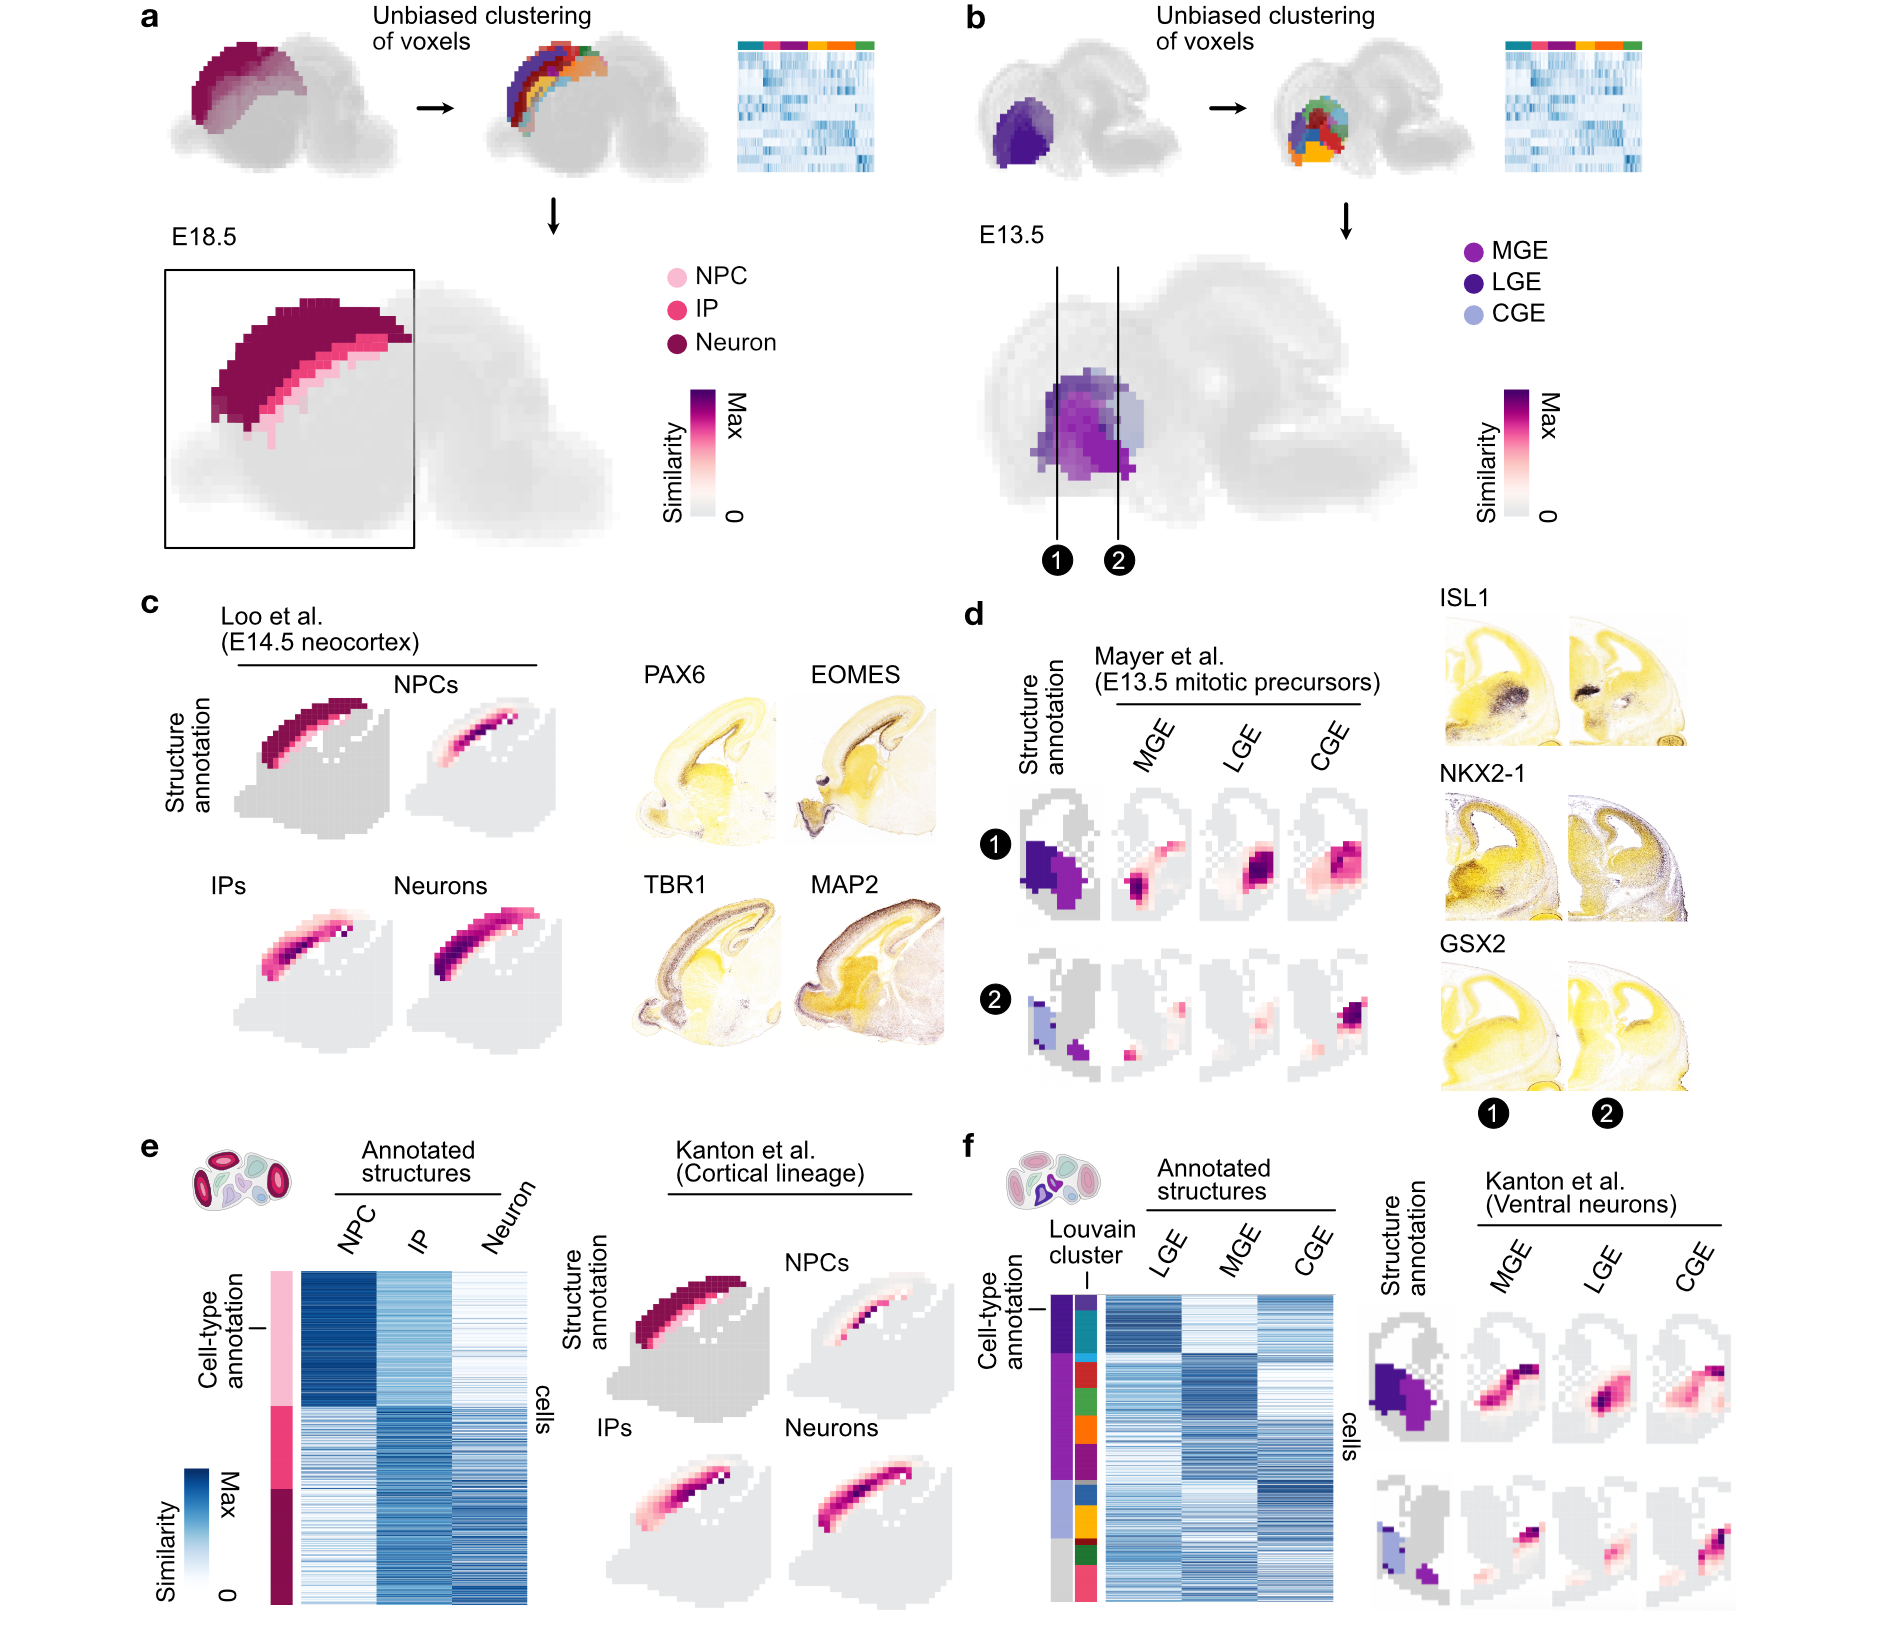
\includegraphics[width=\textwidth]{figures/voxhunt/Figure_5}
    \caption{\textbf{Substructure resolution of transcriptomic maps.} (A and B) Schematic of substructure annotation. Unbiased clusters of voxels were annotated based on the expression of canonical marker genes to identify fine structures beyond existing annotations in the dorsal (A) and ventral (B) telencephalon. (C) Left: sagittal sections visualizing custom substructure annotations and scaled similarity scores from E14.5 mouse neocortex NPC, IP, and neuron primary scRNA-seq data to voxel maps of the E18.5 mouse brain. Right: ISH images of marker gene expression in shown sections. (D) Left: coronal sections visualizing custom substructure annotations and scaled similarity scores from E13.5 mouse mitotic precursors from LGE, MGE, and CGE primary scRNA-seq data (Mayer et al., 2018) to voxel maps of the E13.5 mouse brain. Right: E13.5 mouse ISH images of marker gene expression in shown sections. (E) Left: heatmap showing similarities of cortical cells from cerebral organoids (Kanton et al., 2019) to annotated substructures. Right: coronal sections visualizing custom annotations and scaled similarity scores from organoid cell states to voxel maps of the E13.5 mouse brain. LGE, MGE, and CGE, lateral, medial, and caudal ganglionic eminence; NPC, neural progenitor cell; IP, immediate progenitor. (F) Left: heatmap showing similarities of ventral neurons from cerebral organoids (Kanton et al., 2019) to annotated substructures and their resulting annotations. Right: coronal sections visualizing custom annotations and scaled similarity scores from organoid ventral neuron populations to voxel maps of the E13.5 mouse brain.}
    \label{fig:vox5}
\end{figure}

\clearpage

\topparagraph{Spatial mapping of chromatin accessibility data}
Next, we show that similar analyses can be performed for single-cell ATAC-seq (Assay for Transposase-Accessible Chromatin using sequencing) data. In this case, we obtained paired scATAC-seq and scRNA-seq data performed on the same cell suspension generated from micro-dissected regions from 2-4 month cerebral organoids (\cite{kanton_organoid_2019}) (Figure 2.6a). We determined accessibility scores at the transcription start site (TSS) of each gene measured in the in situ hybridization atlas (Figure 2.6b), and then calculated TSS access and expression correlation across each structure annotated in the voxel map (Figure 2.6c,d). Coloration of the 3D voxel map based on correlation revealed that both transcriptomes and chromatin accessibility scores of neuronal cells from the micro-dissected region have the highest correlation with the developing cortex (Figure 2.6e). This demonstrates that VoxHunt can annotate cells across multiple single-cell -omics modalities.

\begin{figure}[b!]
    \centering
	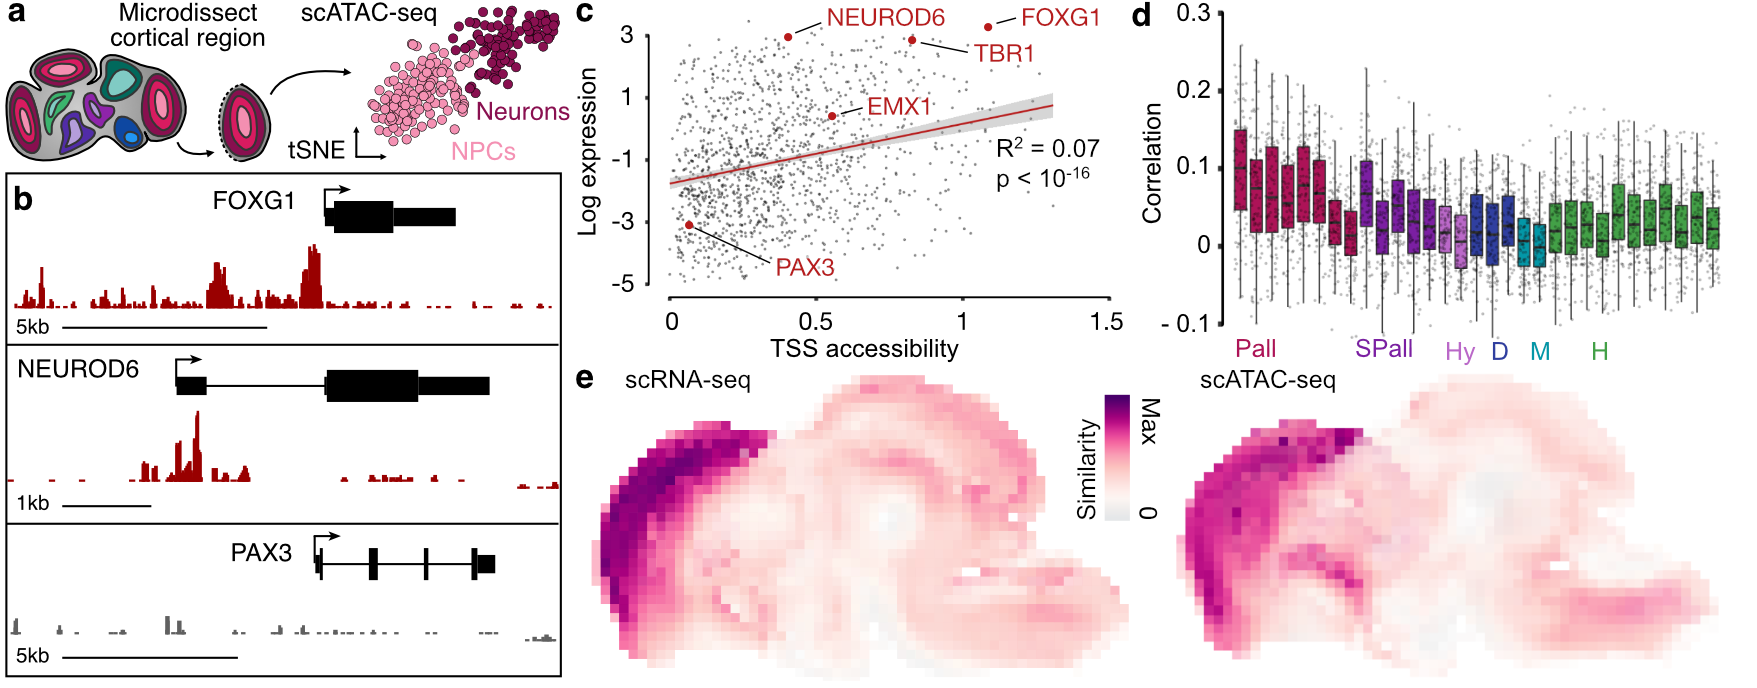
\includegraphics[width=\textwidth]{figures/voxhunt/Figure_6}
    \caption{\textbf{Projecting chromatin accessibility profiles to spatial brain maps.} (A) Single-cell RNA-seq (Camp et al., 2015; Kanton et al., 2019) and single-cell ATAC-seq (Kanton et al., 2019) was performed on single cortical regions microdissected from cerebral organoids between 2 and 4 months of age. (B) Signal tracks showing accessibility (normalized read count) at the transcription start site (TSS) of the forebrain marker FOXG1, the cortex neuron marker NEUROD6, and the hindbrain marker PAX3. (C) Expression of all measured genes in the E13.5 pallium (cortex) as a function of TSS accessibility in cortical organoid cells. The fit of a linear model is indicated in red, the gray area shows the standard error, and the indicated p-value was obtained through an F-test. (D) Boxplots showing Pearson correlation distributions of organoid TSS accessibility (log-normalized peak count) to gene expression in different brain structures. (E) Sagittal projections of the E13.5 mouse brain colored by scaled similarity scores of organoid TSS accessibility (scATAC-seq) or expression (scRNA-seq) with voxel map expression of the downstream gene. Pall, pallium; SPall, subpallium; Hy, hypothalamus; D, diencephalon; M, midbrain; H, hindbrain.}
    \label{fig:vox6}
\end{figure}

\topparagraph{Reference-based deconvolution of organoid bulk transcriptomes}
There are on-going efforts to steer brain organoid development toward distinct regional identities by supplying cues in defined culture conditions. Whole organoid bulk transcriptome measurements provide a high-information content metric of organoid states at relative low cost and high throughput. Therefore, we established a framework within VoxHunt to assess organoid brain structure representation using bulk transcriptomics. The pseudo-bulk data can be accurately deconvoluted into proportions of brain regions that are represented within heterogeneous cerebral organoids, and this is further validated with data from directed patterning into cortex or thalamus (Figure S2.7a,b). We note that this approach is particularly powerful at organoid stages where neurons are abundant, as neurons harbor strong structure-specific multi-gene signatures.


\topparagraph{Assessing organoid patterning using multiplexed transcriptomics and reference mapping}
Finally, we highlight how reference-mapping organoid transcriptomes can be used to assess the outcome of culture condition manipulations. We performed a proof of principle experiment where we incubated developing organoids with several different patterning molecules including R-spondin (RSPO) 2, RSPO 3, sonic hedgehog (SHH), an activator of the Wnt pathway (CHIR99021), and two small molecules for dual SMAD inhibition (SB431542, Dorsomorphin) (Figure 2.7a; S7c). We generated organoids in a multi-well plate and performed bulk RNA sequencing of multiple individual organoids after transient treatment with two concentrations of each of these molecules, as well as control untreated organoids, resulting in 61 total bulk transcriptome measurements. Principal component analysis (PCA) showed transcriptome heterogeneity induced by morphogen treatment that were largely consistent across organoids for a given condition (Figure 2.7b). Next, we correlated each bulk transcriptome to each voxel within the ABA developing mouse brain reference (E11.5), and found variation between conditions that was consistent across organoids for a given condition (Figure 2.7c). Interestingly, we found that RSPO2 and RSPO3 conditions had similar and reproducible patterns with enriched mapping to a particular location within the developing brain. As noted above, RSPO2/3 expression localizes to the invaginated telencephalic roof plate (\cite{kamata_r-spondin_2004}) and transient structures annotated as pallium at the boundary of the developing telencephalon and diencephalon (Figure S2.6d,e). The RSPO2/3-induced signature in organoids was distinct from control organoids as assessed through PCA and differential expression analysis (Figure 2.7b,d-e). The locations with highest mapping of the RSPO2/3 treated organoids were voxels adjacent to where both of these genes are highly and specifically expressed in the developing brain (Figure 2.7f,h). In addition, many genes that are differentially expressed between control and RSPO2/3- treated organoids are also expressed in voxels adjacent to the RSPO2/3 positive location, including choroid plexus markers TTR, CLU, and HTR2C (Figure 2.7f-h). It is unclear how RSPO2/3 might induce choroid plexus formation, and known R-spondin receptors such as Leucine-rich repeat-containing G-protein-coupled receptors (LGRs) are not probed for in the ABA. Nonetheless, this data provides a potential hint into how local morphogen expression within the developing brain might impact the development of cell phenotypes within neighboring structures. Altogether, this experiment provides an experimental and computational strategy for modulating and assessing developing brain organoids in high-throughput through transcriptome sequencing and reference atlas comparison.


\begin{figure}[t!]
    \centering
	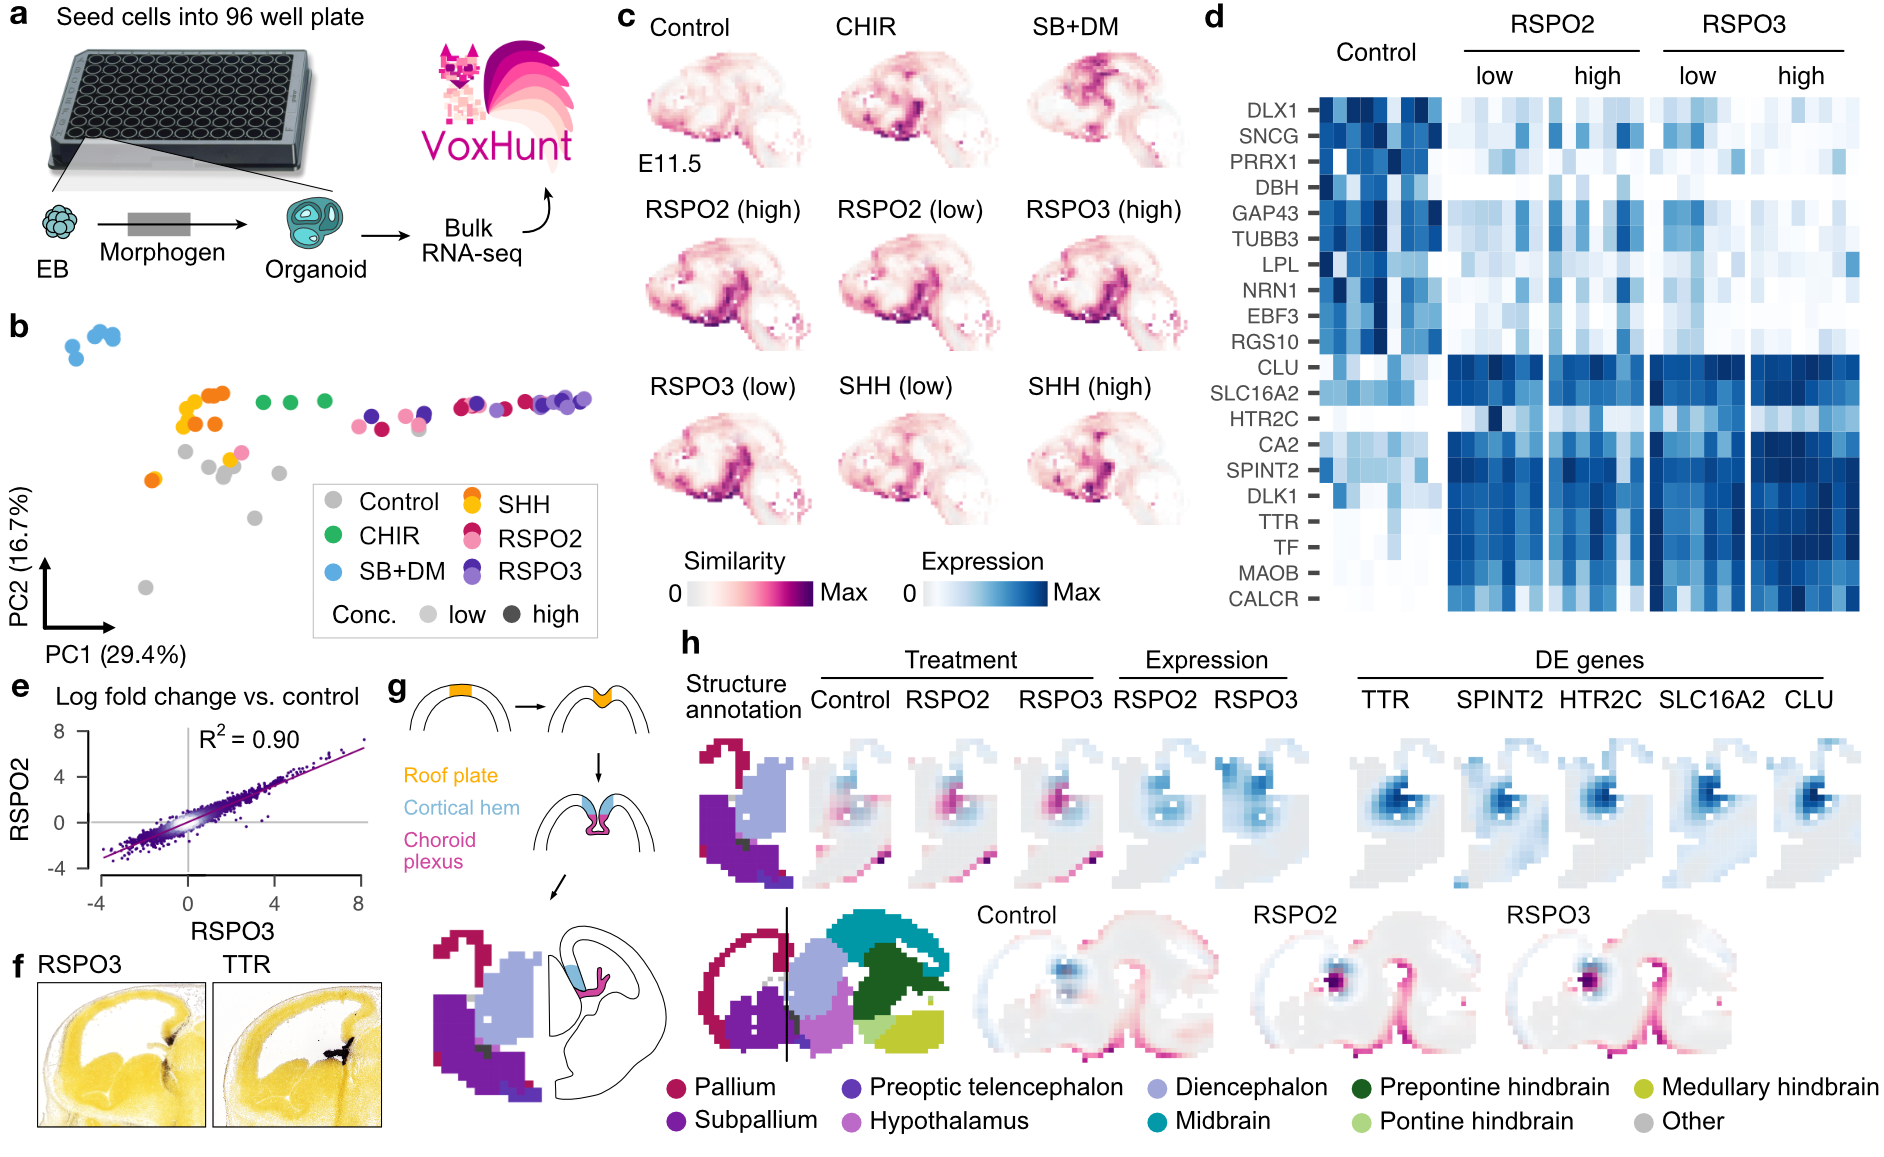
\includegraphics[width=\textwidth]{figures/voxhunt/Figure_7}
    \caption{\textbf{Assessing the effects of morphogens on brain organoids using multiplexed bulk transcriptomics.} (A) Schematic of the experimental setup. Single developing organoids were exposed to different morphogens in a 96-well plate. Bulk RNA-seq libraries were prepared from each organoid and multiplexed for sequencing. (B) First two principal components of organoid transcriptomes. Each point represents one individual organoid and is colored by condition. (C) Spatial similarity maps of each condition to the E11.5 developing mouse brain ISH atlas. (D) Heatmap showing the expression of differentially expressed genes between control and R-spondin conditions.(E) Correlation of transcriptomic effect sizes (log fold change) for RSPO2 and RSPO3 conditions compared to control samples. (F) In situ hybridization images of RSPO3 and the choroid plexus marker TTR in coronal sections of E13.5 mouse brain. (G) Schematic of roof plate invagination and early stages of choroid plexus development. (H) Top left: coronal sections visualizing regional annotation and scaled similarity scores overlaid with RSPO3 expression for control and R-spondin conditions. Top right: coronal sections visualizing expression of differentially expressed genes between control and R-spondin conditions. Bottom: sagittal sections visualizing the regional annotation and scaled similarity scores overlaid with RSPO3 expression for control and R-spondin conditions.}
    \label{fig:vox7}
\end{figure}



\subsection{Discussion}
Here we have developed a set of computational tools that enables researchers to quickly and flexibly explore the vast amount of data within the Allen Brain Atlas and other brain reference resources. We provide multiple examples for how these tools can be implemented to interpret single-cell genomic data from 3D brain tissue cultures through systematic comparison to these references. There are still many uncertainties about how to effectively generate brain structures from humans and other species in vitro. VoxHunt \href{https://github.com/quadbiolab/voxhunt}{https://github.com/quadbiolab/voxhunt} will be a powerful approach to assess organoid engineering protocols, to annotate cell fates that emerge in organoids during genetic and environmental perturbation experiments, and to develop data-driven hypotheses about the mechanisms underlying mammalian brain patterning that can be tested in vitro. 

\topparagraph{Limitations of the study}
One major limitation with the current VoxHunt implementation is that the most comprehensive brain transcriptome atlases have been generated using mouse brain tissue. The human brain has evolved features that are different from other mammals and primates, and there are certain scenarios where comparison to non-human tissues may be inadequate. In addition, single-cell sequencing has illuminated a great diversity of molecularly distinct neuronal and non-neuronal states in the brain, which is partially recapitulated in engineered human brain tissues. However, there is not yet a comprehensive spatial reference with single cell resolution across the entire brain to use a query space for organoid-reference comparisons. High-resolution 4D reference brain maps will serve as valuable resources for unbiased and high-dimensional search spaces, and VoxHunt will be an important tool to explore and interpret bulk and single-cell sequencing data from brain organoid systems. 


\subsection{Methods}

\paragraph{Acknowledgments}
We thank the Treutlein and Camp labs for helpful discussions and Sophie Jansen and Ryoko Okamoto for experimental support. We also want to thank the Kirkeby lab for kindly sharing the NKX2.1GFP/w cell line. This project was made possible in part by the Chan Zuckerberg Initiative DAF (grant CZF2017-173814 to J.G.C. and B.T.), a Silicon Valley Community Foundation advised fund, the European Research Council (Anthropoid-803441 to J.G.C. and Organomics-758877 and Braintime-874606 to B.T.), the Swiss National Science Foundation (project grant 310030\_84795 to J.G.C. and project grant 310030\_192604 to B.T.), and the National Center of Competence in Research, Molecular Systems Engineering. J.S.F. was supported by a Ph.D. fellowship of the Boehringer Ingelheim Fonds.

\paragraph{Author contributions}
J.S.F. developed the computational tool and performed computational analyses with support from Z.H. and M.J.B. F.S.C. designed and executed the patterning experiment with assistance from M.S. J.S.F., F.S.-C., B.T., and J.G.C. designed the study and wrote the manuscript.

\paragraph{Declaration of interests}
B.T. is a member of the Cell Stem Cell advisory board.

\paragraph{Data and code availability}
VoxHunt was implemented as an R package and is available at\\\href{https://github.com/quadbiolab/voxhunt}{https://github.com/quadbiolab/voxhunt}. \\
R markdown scripts reproducing the main analyses in study are available at\\ 
\href{https://github.com/quadbiolab/voxhunt_reproducibility}{https://github.com/quadbiolab/voxhunt\_reproducibility}.\\
All datasets used in this study are available for download in public repositories (see Key Resources Table for individual accession numbers). 

\paragraph{Materials availability}
HES3, NKX2.1GFP/w hESCs will be provided upon execution of a suitable Materials Transfer Agreement (MTA) with Ed Stanley and Andrew G. Elefanty (Murdoch Childrens Research Institute, Melbourne).

\paragraph{hESC experiments approval}
Stem cell experiments with NKX2.1GFP/w hESCs were approved by the Bundesamt für Gesundheit (Swiss Health Federal Office) with disposition number 606.0000-1/31 / 19.018224; and by the Ethikkommission Nordwest- und Zentralschweiz (Ethics Commision for Northern and Central Switzerland)

\paragraph{hESC Line Culture and Maintenance}
NKX2.1GFP/w hESCs were obtained from Agnete Kirkeby’s research group at the University of Copenhagen, after arrangement of an MTA with Ed Stanley and Andrew G. Elefanty (Murdoch Childrens Research Institute, Melbourne). NKX2.1GFP/w hESCs were grown at 37oC, 5\% CO2 in feeder-free conditions, on 6-well tissue culture plates coated with hESC-Qualified Matrigel (Corning). hESCs were fed every other day with mTesR Plus (StemCell Technologies) and passaged when reaching around 80\% confluence with EDTA for gentle dissociation. NKX2.1GFP/w hESCs were tested at passage 67 for copy number changes using the Agilent ISCA 8x60K v2 array and no abnormalities were detected. Cells were also karyotyped at passage 78 and showed apparently normal female karyotype in 20 cells examined. These analyses were performed by the Cell Guidance Systems Genetics Service (Cambridge, UK). Regular PCR-based Mycoplasma testing (Biological Industries) was performed to discard potential Mycoplasma infections.

\topparagraph{Brain organoid generation and incubation with patterning molecules}
NKX2.1GFP/w hESCs (passage 69) were trypsinized using TrypLETM Express Enzyme (Thermo Fisher Scientific) to obtain single cell suspensions and 500 cells were plated in each well of ultra-low attachment 96-well plates (day 0). Cells in suspension were cultured for one day in mTesR Plus (StemCell Technologies) to allow for aggregation and Embryoid Body (EB) formation. On day 1, EBs were transitioned to Neural Induction Media (NIM, containing DMEM/F12, 1\% N2 supplement (v/v), 1\% GlutaMAX supplement (v/v), 1\% MEM-NEAA (v/v) and 1 µg/mL Heparin). From day 3 to day 6, organoids were incubated in Neural differentiation media (Ndiff-VA, ½ DMEM/F1, ½ Neurobasal, 0.5\% N2 supplement (v/v), 1\% B27 supplement without Vitamin A (v/v), 1:4000 insulin (Sigma Aldrich), 49.5 µM 2-Mercaptoethanol, 1\% GlutaMAX (v/v) (Invitrogen), 0.5\% MEM-non essential amino acids and 1\% Penicillin/Streptomycin). Finally, organoids were transferred to Neural Maturation Media (Ndiff+VA, same recipe as Ndiff-VA but with B27 supplement containing Vitamin A) on day 6 and media was changed every 2-3 days until day 14. Matrigel was added to the corresponding media at increasing dilutions during organoid development. From day 3 to 6, brain organoids were supplemented with 1:50 Growth Factor Reduced (GFR) Matrigel (Corning); from day 6 to 8, with 1:100 GFR Matrigel; and from then on with 1:200 GFR Matrigel. Patterning factors were added in low and high concentrations from day 3 to 6: SHH (low, 50 ng/mL; high, 100 ng/mL), RSPO2 (low, 100 ng/mL; high, 1 µg/mL), RSPO3 (low, 100 ng/mL; high, 1 µg/mL), SB-431542 and Dorsomorphin (1 µM and 2.5 µM, respectively) and CHIR (low, 0.5 µM; high, 5 µM).  

\paragraph{Collection of patterned organoids and RNA purification}
On day 14, all culture media was removed and patterned brain organoids were snap-frozen in a bed of isopentane (Sigma-Aldrich) and dry ice. Immediately following freezing, organoids were transferred to -80˚C and stored at this temperature until the day prior to RNA extraction. On that day, organoids were immersed in 200 µl of RNA Later ICE (Thermo Fisher) and defrosted overnight to protect RNA from degradation during the following steps. Organoids were transferred to TriReagent  (Thermo Fisher) and immediately vortexed for 30 seconds to homogenize the tissue. After 5 minutes of incubation at room temperature, 0.1X volumes of 1-Bromo-3-chloropropane (BCP, Lucerna-Chem) were added, followed by a 10 second-vortexing step and 5 minutes of incubation at room temperature. Samples were centrifuged at 12,000g for 10 minutes (4˚C) and 100 µL of supernatant (aqueous phase) was collected to proceed with RNA purification using the spin procedure of the MagMax-96 total isolation kit (Thermo Fisher). 

\paragraph{Smartseq2 library preparation}
Purified bulk RNA samples from each individual\\organoid were then processed for Smartseq2 (SS2) library generation using the protocol published by Picelli and colleagues (Picelli et al., 2014) with slight modifications. As our starting material was extracted RNA and not single cells, Triton X-100 in lysis buffer was replaced by Nuclease-Free water. Therefore, lysis buffer composition was 1:10 RNase inhibitor (Takara) in Nuclease-free water (Invitrogen). 1 µl of extracted bulk RNA was incubated with 1 µL of lysis buffer, 1 µL of oligo-dT primer and 1 µL of dNTP mix (Thermo Fisher Scientific) for 3 minutes at 72 oC.
Next, samples were reverse transcribed using the SuperScript II kit with DTT (Thermo Fisher Scientific). The RT mix included 100 U SuperScript II, 10 U RNAse inhibitor (Takara), 1X First-Strand buffer, 5 mM DTT, 1 µM Template-Switch Oligo (TSO), 1 M Betaine (Sigma-Aldrich) and 6 mM MgCl2 (Sigma-Aldrich) previously diluted in Nuclease-Free water (Invitrogen). Samples were incubated at 42oC for 90 min, followed by 10 cycles at 50oC for 2 min and 42oC for 2 min to prevent secondary RNA structures from stopping the polymerase and enable completion of RT. Finally, samples underwent an enzyme inactivation step at 70oC for 15 minutes.
Next, a PCR preamplification step (SS2 PCR) was performed. The PCR mix contained 10 µL of reverse-transcribed sample, 1X KAPA HiFi HotStart ReadyMix (Roche), 0.1 µM IS PCR primers (IDT) and Nuclease-Free water (Invitrogen) up to a total volume of 25 µL. PCR was performed using the following program: initial denaturation step at 98oC for 3 min, 15 cycles of 98oC for 20 s - 67oC for 15 s - 72oC for 6 min, and a final elongation step at 72oC for 5 min.
SS2 reactions were cleaned up using AMPure XP reagent (Beckman Coulter) at 1X ratio and subsequently quality-checked for fragment sizes and concentrations with Qubit 2.0 (Invitrogen) and Agilent 2100 Bioanalyzer (Agilent Technologies). All samples were then adjusted to concentrations around 200 pg/µL with EB solution (Qiagen) prior to Nextera library preparation.
Tagmentation of cDNA was performed at 55oC for 5 min, using the Nextera XT DNA sample preparation kit (Illumina). Each tagmentation reaction was composed of 2.5 µL (1X) Tagment DNA (TD) buffer, 1.25 µL Amplicon Tagment Mix (ATM) and 250 pg (around 1.25 µL) of purified DNA from PCR. Immediately after, Tn5 transposase was stripped off the DNA by incubating each reaction with 1.25 µL of Neutralize Tagment (NT) buffer for 5 min at room temperature. 
A final amplification of tagmented DNA (indexing PCR) was performed with index primers from Set B of Nextera XT Index Kit v2 (Illumina). 1.25 µL of each i5 and i7 adapter and 3.75 µL of Nextera PCR Mastermix (NPM) were added to 1.25 µL of each sample prior to running the indexing PCR with Illumina’s recommended settings: extension at 72oC for 3 min, denaturation at 95oC for 30 s, 12 cycles of 95oC for 10 s - 55oC for 30 s - 72oC for 30 s, and a final elongation step at 72oC for 5 min.
Immediately after indexing PCR, samples were pooled in equal ratios by adding 3 µL of each sample to a 1.5 mL tube. Pooled libraries were then cleaned up twice with AMPure XP (Beckman Coulter) at 0.9X ratio. Of note, a 0.9X ratio of AMPure XP was used instead of 1X ratio (as stated in Picelli et al., 2014) because it proved more efficient removing small carryover primers. A final quality control with Qubit 2.0 (Invitrogen) and Agilent 2100 Bioanalyzer (Agilent Technologies) showed cDNA concentration in the range of 10 nM.

\paragraph{Sequencing of SS2 libraries}
The pooled libraries were appropriately diluted and sequenced at the Genomics Facility Basel (GFB) using NextSeq, with paired-end configuration and 38 cycles. Sequencing data was demultiplexed by the GFB, using bcl2fastq version 2.20.422 with the following parameters: --ignore-missing-bcls --ignore-missing-controls --ignore-missing-positions --ignore-missing-filter --no-bgzf-compression --barcode-mismatches 1.
 
\paragraph{Acquisition and preprocessing of Allen Brain Atlas in situ hybridization data}
We downloaded 3D expression grid data from all in situ hybridization (ISH) experiments corresponding to the eight developmental time points (E11.5, E13.5, E15.5, E18.5, P4, P14, P28, P56) using the application programming interface (API) provided by the Allen Brain Atlas (ABA) Developing Mouse Brain Data Portal (http://help.brain-map.org/display/devmouse/API). In order to obtain in situ intensity profiles (all genes) for each voxel, the data for each timepoint was summarized into a voxel by gene matrix. If multiple experiments were available for the same gene and time point, we calculated the arithmetic mean across experiments. To be able to perform comparisons to human transcriptomics data, we converted the gene names (official gene symbols) to the names of the human homolog, using homology annotations from the Mouse Genome Informatics database (http://informatics.jax.org). Genes without a human homolog were excluded from the dataset. The structure ontology was obtained by downloading the structure graph with ID 17 through the ABA web API (http://api.brain-map.org/). The resulting json file was converted into a data frame. For differential expression testing and visualization, we introduced four additional levels of annotation by summarizing existing annotations. In these custom annotations, pallium (dorsal forebrain), subpallium (ventral forebrain), hypothalamus, diencephalon, midbrain, hindbrain and spinal cord are on the same level on the ontology tree and each splits further into finer structures. For the analysis shown here as well as for the VoxHunt package, we removed all voxels annotated as spinal cord, as this structure was only included in the earliest developmental stages. To remove background signal from in situ hybridization intensities we applied a minimum intensity threshold of 1. The final expression matrices including metadata and custom annotations can be found as RDS files under http://doi.org/10.17632/g4xg38mwcn.1. 

\paragraph{Visualization of the structure annotation ontology}
To visualize the structure ontology as a tree, we used the data.tree R package (Glur, 2020) to convert the structure ontology data frame into a phylo object. We used the tidytree R package (Yu, 2020) to manipulate the tree and add custom annotations to the nodes. Finally, the tree was plotted with the ggtree R package (Yu, 2020) using a circular layout and edges were colored according to our custom annotation level 3. 
 
\paragraph{Acquisition of organoid single-cell gene expression and chromatin accessibility data}
With the goal of covering a range of different organoid protocols, we collected published single cell gene expression data from dorsal forebrain (Birey et al., 2017; Velasco et al., 2019), ventral forebrain (Birey et al., 2017; Xiang et al.) thalamus (Xiang et al., 2019), and cerebral (Kanton et al., 2019) (unpatterned) organoids. Single cell gene expression and/or chromatin accessibility data for these organoids was obtained through the following GEO accessions: GSE93811 for Birey et al. (cortical and ventral), GSE97882 for Xiang et al. (ventral), and GSE122342 for Xiang et al. (thalamus) and the following ArrayExpress accessions: E-MTAB-7552 for Kanton et al. (cerebral scRNA-seq) and E-MTAB-8089 for Kanton et al. (cerebral scATAC-seq). 

\paragraph{Acquisition of primary bulk and single-cell gene expression data}
We obtained a single-cell gene expression atlas from the developing mouse brain (La Manno et al., 2020) from the Mouse Brain Atlas website (\href{http://mousebrain.org/downloads.html}{http://mousebrain.org/downloads.html}). Average cluster transcriptomes and annotations were obtained from the file dev\_all.agg.loom and tSNE embedding coordinates for and annotations for individual cells were obtained from the file dev\_all.loom. In addition, we obtained single-cell gene expression data (split-pool barcoding) from the developing mouse brain (Rosenberg et al., 2018) through the GEO accession GSE110823. From the dataset, we extracted one representative neuronal cluster for each evaluated structure: “OB mitral/Tufted Ms4a15” for olfactory bulb, “Medium Spiny Neurons” for striatum, “CTX PyrL6a” for cortex, “MTt Glut” for rostral midbrain, “THAL Glut” for thalamus, “Purkinje Late” for cerebellum, “MD Int Rxfp2” for medulla and “HIPP Granule Nrp2” for hippocampus. Single-cell gene expression data from the mouse ganglionic eminences (Mayer et al., 2018) was obtained through the GEO accession GSE104158 and we extracted ‘mitotic precursors’ annotated as CGE, LGE and MGE for our analysis. Single-cell gene expression data from the developing mouse neocortex (Loo et al., 2019) was obtained from the GEO accession GSE123335. Bulk RNA-seq data from microdissected regions of the human brain was obtained from BrainSpan (\href{http://www.brainspan.org/static/download.html}{http://www.brainspan.org/static/download.html}). We obtained four datasets with single-cell transcriptomic data of the developing human brain through the following GEO accessions: GSE104276 for Zhong et al. (Zhong et al., 2018), GSE10372 for Fan et al. (Fan et al., 2018), the dbGaP accession phs001836.v1.p1 for Polioudakis et al. (Polioudakis et al., 2019) and through the USCS Cell Browser portal (\href{https://cells.ucsc.edu/?ds=cortex-dev}{https://cells.ucsc.edu/?ds=cortex-dev}) for Nowakowski et al. (Nowakowski et al., 2017).  

\paragraph{Preprocessing of single-cell gene expression data}
Transcript count matrices were preprocessed separately for each dataset with consistent parameters using the R package Seurat 3.0 (Stuart et al., 2019). Cells were filtered based on unique molecular identifier (UMI) counts (>500, <50000), the number of detected genes (>200, <6000) and the fraction of mitochondrial genes (<0.1). For all datasets, we annotated cells based on the cell type labels from the original paper and filtered out unannotated cells. Counts for each cell were normalized by the total number of counts for that cell, multiplied by a scaling factor of 10000 and subsequently natural-log transformed (NormalizeData()). Log normalized expression values were used as an input to the function FindVariableFeatures() to find the 2000 most variable genes based on the ‘vst’ selection method. Expression levels of these genes were used to perform Principal Component Analysis (PCA) with the function prcomp\_irlba() from the irlba R package (Jim Baglama, 2019) and the top 15 principal components (PCs) were used to produce a two-dimensional embedding with Uniform Manifold Approximation and Projection (UMAP) (Becht et al., 2019). 

\paragraph{Differential expression analysis of ISH and single-cell data}
To perform differential expression analysis (DE) on both ISH and single-cell expression data, we calculated the Wilcoxon rank sum test p-values with a Benjamini-Hochberg multiple testing correction (q-value), AUROC values and log fold changes using the wilcoxauc() function from the R-package presto (Korsunsky et al., 2019). For the ISH data, we first performed DE on log2-transformed intensity values with a pseudocount of 1x10-10 between custom annotation levels filtered for statistical significance (q < 10-5) and sorted by AUROC value to find highly specific marker genes for each structure (structure markers). To find time point-specific genes, we further performed DE between developmental stages for each structure on custom annotation level 2 separately (stage markers). Additionally, we searched for genes whose expression in a structure is upregulated at any fetal developmental stage and is maintained in subsequent stages. For fetal stages E13.5, E15.5 and E18.5 we performed DE between the current stage and all, and older stages versus all younger stages (e.g. for genes upregulated at E15.5: E11.5 and E13.5 vs E15.5 and E18.5) for each structure on custom annotation level 2 separately (fetal development markers). For single-cell data, we performed DE on log normalized expression levels between annotated cell types for each dataset separately. Here, we determined unbiased cluster markers by taking 3 statistically significant (q < 10-5) genes with highest log fold change for each cluster. 

\paragraph{Correlation of single-cell transcriptomes to brain structures}
To determine best matching brain structures for each neuronal cluster in the organoid datasets, we calculated the correlation of single cell transcriptomes with gene expression of structures in the fetal E13.5 mouse brain. For each cell in each cluster we calculated the Pearson correlation coefficient between the log normalized transcript count for each cell and the expression vector of each voxel in the E13.5 mouse brain based on 189 structure marker genes (top 10 for each structure at level 3). Correlation coefficients for each cell were then summarized for each structure by calculating the arithmetic mean. From the mean correlation coefficient of each cell with each structure we then defined the similarity to the structure as 


\[
s_{ij} = 
\begin{cases}
    r_{ij}, & \text{if } r_{ij} > 0\\
    0,              & \text{otherwise}
\end{cases}
\]

We assigned each cell to the structure with maximum similarity and displayed the mean similarity to each structure for all clusters. 
  
\paragraph{Calculation of similarity to developmental stages}
To assess the relationship between the age of the neuronal population and the mouse developmental stage, we calculated for each cell in each neuronal population the highest correlating voxel in the best matching structure of custom annotation level 2 for this population. We selected genes that were informative with regard to the developmental stage for each structure separately by taking the union of the above mentioned fetal development markers (top 50 AUROC for each stage and structure) and stage markers specific to E11.5 (top 50 AUROC for each structure) and used their expression values as an input for computing the above described similarity based on Pearson correlation. In total, this resulted in 183 genes for the pallium, 181 genes for the subpallium, 179 genes for the midbrain and 181 genes for the diencephalon. 

\paragraph{Evaluating the effect of feature selection and downsampling}
To test how size of the feature set and data quality affect the fidelity of the mapping, we used VoxHunt to map single-cell transcriptome data from the P2 mouse brain (Rosenberg et al., 2018) to voxel maps of the P4 mouse brain and evaluated its performance under different conditions. First, we extracted various feature sets from the P4 mouse brain voxel maps. In the case of DE genes, we adjusted the size of the feature set by taking the 1, 5, 10, 20, 30, 50 or 200 most specific genes for each structure at custom annotation level 3. In the case of variable features, we selected the 10, 50, 100, 200, 500 or 1000 most variable genes. For each feature set as well as for the full set of 1757 genes we computed the similarity of each cell to each structure as described above. For each feature set and brain structure, we evaluated accuracy as the fraction of correctly assigned structures and contrast as the ratio between the similarity to the second best structure and the assigned structure. To evaluate the effect of data quality on the mapping, we further used the function downsampleMatrix() from the R package DropletUtils (Lun et al., 2019) to downsample the UMI counts of the dataset to as low as 10\%. For each downsample fraction and feature set, we computed similarity maps, assigned cells to their most similar structure and computed accuracy as described above.

\paragraph{Spatial correlation maps of organoid cells transcriptomes}
To compute spatial correlation patterns of single-cell transcriptomes to ISH maps, we first intersected the genes measured in the ABA with all genes detected in the dataset. From these genes, we then picked the 10-20 most specific genes for each structure on custom annotation level 3 based on AUROC values to receive 200-300 genes for each dataset (exact feature sets can be found in Supplementary Table 2.1). Based on the expression values of the resulting gene set, we calculated the Pearson correlation coefficient between each cell and each voxel. Correlation coefficients for each cell cluster were summarized by computing the arithmetic mean for each voxel and subsequently transformed to a similarity metric as described above. Scaled correlation values were displayed as similarity maps across the brain in a sagittal view and on coronal sections. To summarize the similarities to discrete brain structures, we computed the arithmetic mean over the correlations to all voxels in this structure. For estimation of brain structure identities, each cell or cell cluster was assigned the structure of the most highly correlated voxel.  For direct cell-to-voxel projection, we further assigned each cell to the voxel with maximum correlation considering the 8 central sections (5-12) in the E13.5 mouse brain.

\paragraph{Comparison of organoid cells transcriptomes to other reference datasets}
To compare organoid single-cell transcriptomes to RNA-seq data from human microdissected brain structures, we selected the top 50 differentially expressed genes for each structure group in the BrainSpan dataset. Based on these genes, we computed the similarity between each cell and each sample in BrainSpan. To perform comparisons to the single-cell transcriptomic atlas of the developing mouse brain, we used the top 20 spatial structure markers extracted from ISH data to compute the similarity of each cell to the mean transcriptome of each cluster in the reference data. We then visualized these similarities using the tSNE embedding of individual cells. 

\paragraph{Substructure resolution of transcriptomic maps}
To annotate brain structures that were not directly included in the ABA structure ontology, we first performed unbiased clustering on voxelized ISH intensities of the higher-level structure (subpallium for ganglionic eminences (GEs) and dorsal pallium for pallial zones). For this, we performed PCA on voxel ISH intensities with all detected genes and used the first 20 PCs as an input for the louvain clustering algorithm (Blondel et al., 2008) (resolution of 2 for subpallium and 6 for dorsal pallium). Next, we annotated the resulting clusters based on canonical marker genes. We validated these annotations through computing spatial similarity maps of mouse scRNA-seq data from populations derived from the respective structures (Mayer et al., 2018) as described above. For the GEs, we used the newly annotated substructures to annotate cerebral organoid cell populations (Kanton et al., 2019) (ventral neurons from the H9 line). For this, we performed PCA on log-normalized transcript counts of the 2000 most variable genes and used the first 20 PCs to perform louvain clustering (Blondel et al., 2008) at a resolution of 1. The clusters were annotated based on their similarity to the annotated substructures. If the similarity patterns were not sufficiently clear, they were annotated as ‘other’. For pallial zones, we used the cell type annotations from the original publication (Kanton et al., 2019) (cortical lineage from the 409b2 line) and computed their similarities to the annotated substructures. In each case, we used the union of top 10 structure markers on custom annotation level 3 as described above and the top 5 makers (based on high AUROC) of each annotated substructure to compute the Pearson correlation (218 genes for GEs and 188 genes for the pallial zones).

\paragraph{Substructure-resolved annotation of ventral neurons across organoid protocols}
To assess and compare the brain structure identity of inhibitory neuron populations from ventral and cerebral organoid protocols, we extracted neuronal clusters from each dataset and performed PCA on the joined dataset using the scaled expression of all transcription factor coding genes. We used Harmony (Korsunsky et al., 2019) with default parameters to integrate all datasets based on the first 10 principal components. In the integrated space, we performed louvain clustering with a resolution of 2 and computed the similarities of these clusters to GE substructures as described above. We treated the similarity of all cells to all voxels as background similarity and computed a z-score for the similarity of each cell to each GE substructure by subtracting the mean of the background similarity and dividing by its standard deviation. Based on this z-score, we determined the correlation threshold corresponding to a p-value of 0.05. All clusters with a median similarity higher than this threshold were annotated with the maximum correlating structure, while all others were annotated as ‘other’. One cluster showed comparably high similarity above the significance threshold to all three substructures and was annotated as ‘unspecified GE’. To find specific genes for each annotated neuronal population, we performed a Wilcoxon rank sum test and selected genes based on statistical significance (q < 10-5) and fold change (top 10).

\paragraph{Spatial correlation maps of organoid cells chromatin accessibility profiles}
To compute correlation coefficients between transcriptome and chromatin accessibility profiles, the latter was summarized for each gene by counting all peaks in its TSS region (TSS ± 3kb) using the R package CHIPseeker (Yu et al., 2015). TSS peak counts were further normalized by the total number of counts for that cell, multiplied by a scaling factor of 10,000 and subsequently natural-log transformed. We further selected the 10 most specific markers for each structure at custom annotation level 3 to obtain a total of 182 genes and used them to compute the Pearson correlation-based similarity between voxel expression values and log normalized gene accessibility scores for each cell as described above.

\paragraph{Preprocessing and analysis of bulk RNA-seq data}
Sequencing reads from each sample were aligned to the human genome (h38-3.0.0) using STAR v2.5.1b (Dobin et al., 2013). Transcript and gene counts were obtained from BAM files using RSEM v1.3.1 (Li and Dewey, 2011). Both tools were run with standard parameters. Gene counts were normalized to counts per million (CPM) by dividing by the total number of reads per sample and multiplying by a scaling factor of 1,000,000. CPM values were subsequently natural-log transformed (log CPM). Principal component analysis was performed based on scaled log CPM values of the 2000 most highly variable genes. Differential expression analysis data was performed with DESeq2 (Love et al., 2014) using the Seurat function FindMarkers(), followed by a Benjamini-Hochberg multiple testing correction (q-value). To find genes which drive the differences in spatial similarity patterns between condition and control, we selected genes with high statistical significance (q < 10-5) that were measured in the ABA. Out of the resulting gene set, we selected genes with the highest fold change for each direction separately. To compute spatial similarity maps, we used log CPM values of the top 20 structure markers on custom annotation level 3. 

\paragraph{Deconvolution of organoid pseudo-bulk RNA-seq data}
Pseudo-bulk transcriptomes for each organoid were obtained from UMI counts by taking the arithmetic mean of each gene. From the resulting gene expression vector, log CPM values were obtained by dividing by the total number of reads per sample, multiplying by a scaling factor of 1,000,000 and natural-log transformation. For deconvolution based on the Developing Mouse Brain Atlas, ISH fluorescence intensities were analogously transformed to ‘pseudo-CPM’ by log-normalization of each voxel and subsequently summarized for each structure at custom annotation level 2 by calculating the arithmetic mean to obtain transcriptomic references for deconvolution. We used the mean transcriptomes of ‘pallium’, ‘subpallium’, ‘hypothalamus’, ‘diencephalon’, ‘midbrain’, ‘prepontine hindbrain’ and ‘pontine hindbrain’ as references for deconvolution. To perform deconvolution based on bulk RNA-seq data from BrainSpan, we summarized log-normalized counts of all samples aged 12 - 20 pcw to structure groups by calculating the arithmetic mean and used the resulting gene expression vectors as references for deconvolution. Deconvolution of pseudo-bulk organoid transcriptomes was done using EPIC (Racle et al., 2017) for both references separately. We constrained the input to the top 50 level 2 structure markers and used the top 20 level 2 structure markers as ‘sigGenes’. Additionally, we set ‘withOtherCells’ to False and used otherwise default parameters. The estimated structure proportions were further summarized to higher level structures ‘pallium’, ‘ventral telencephalon’ (subpallium and hypothalamus), ‘diencephalon’, and ‘non-telencephalon’ (midbrain and hindbrain).

\clearpage

\subsection{Supplement}
\beginsupplement

\topparagraph{Supplementary Figures}

\begin{figure}[h!]
    \centering
	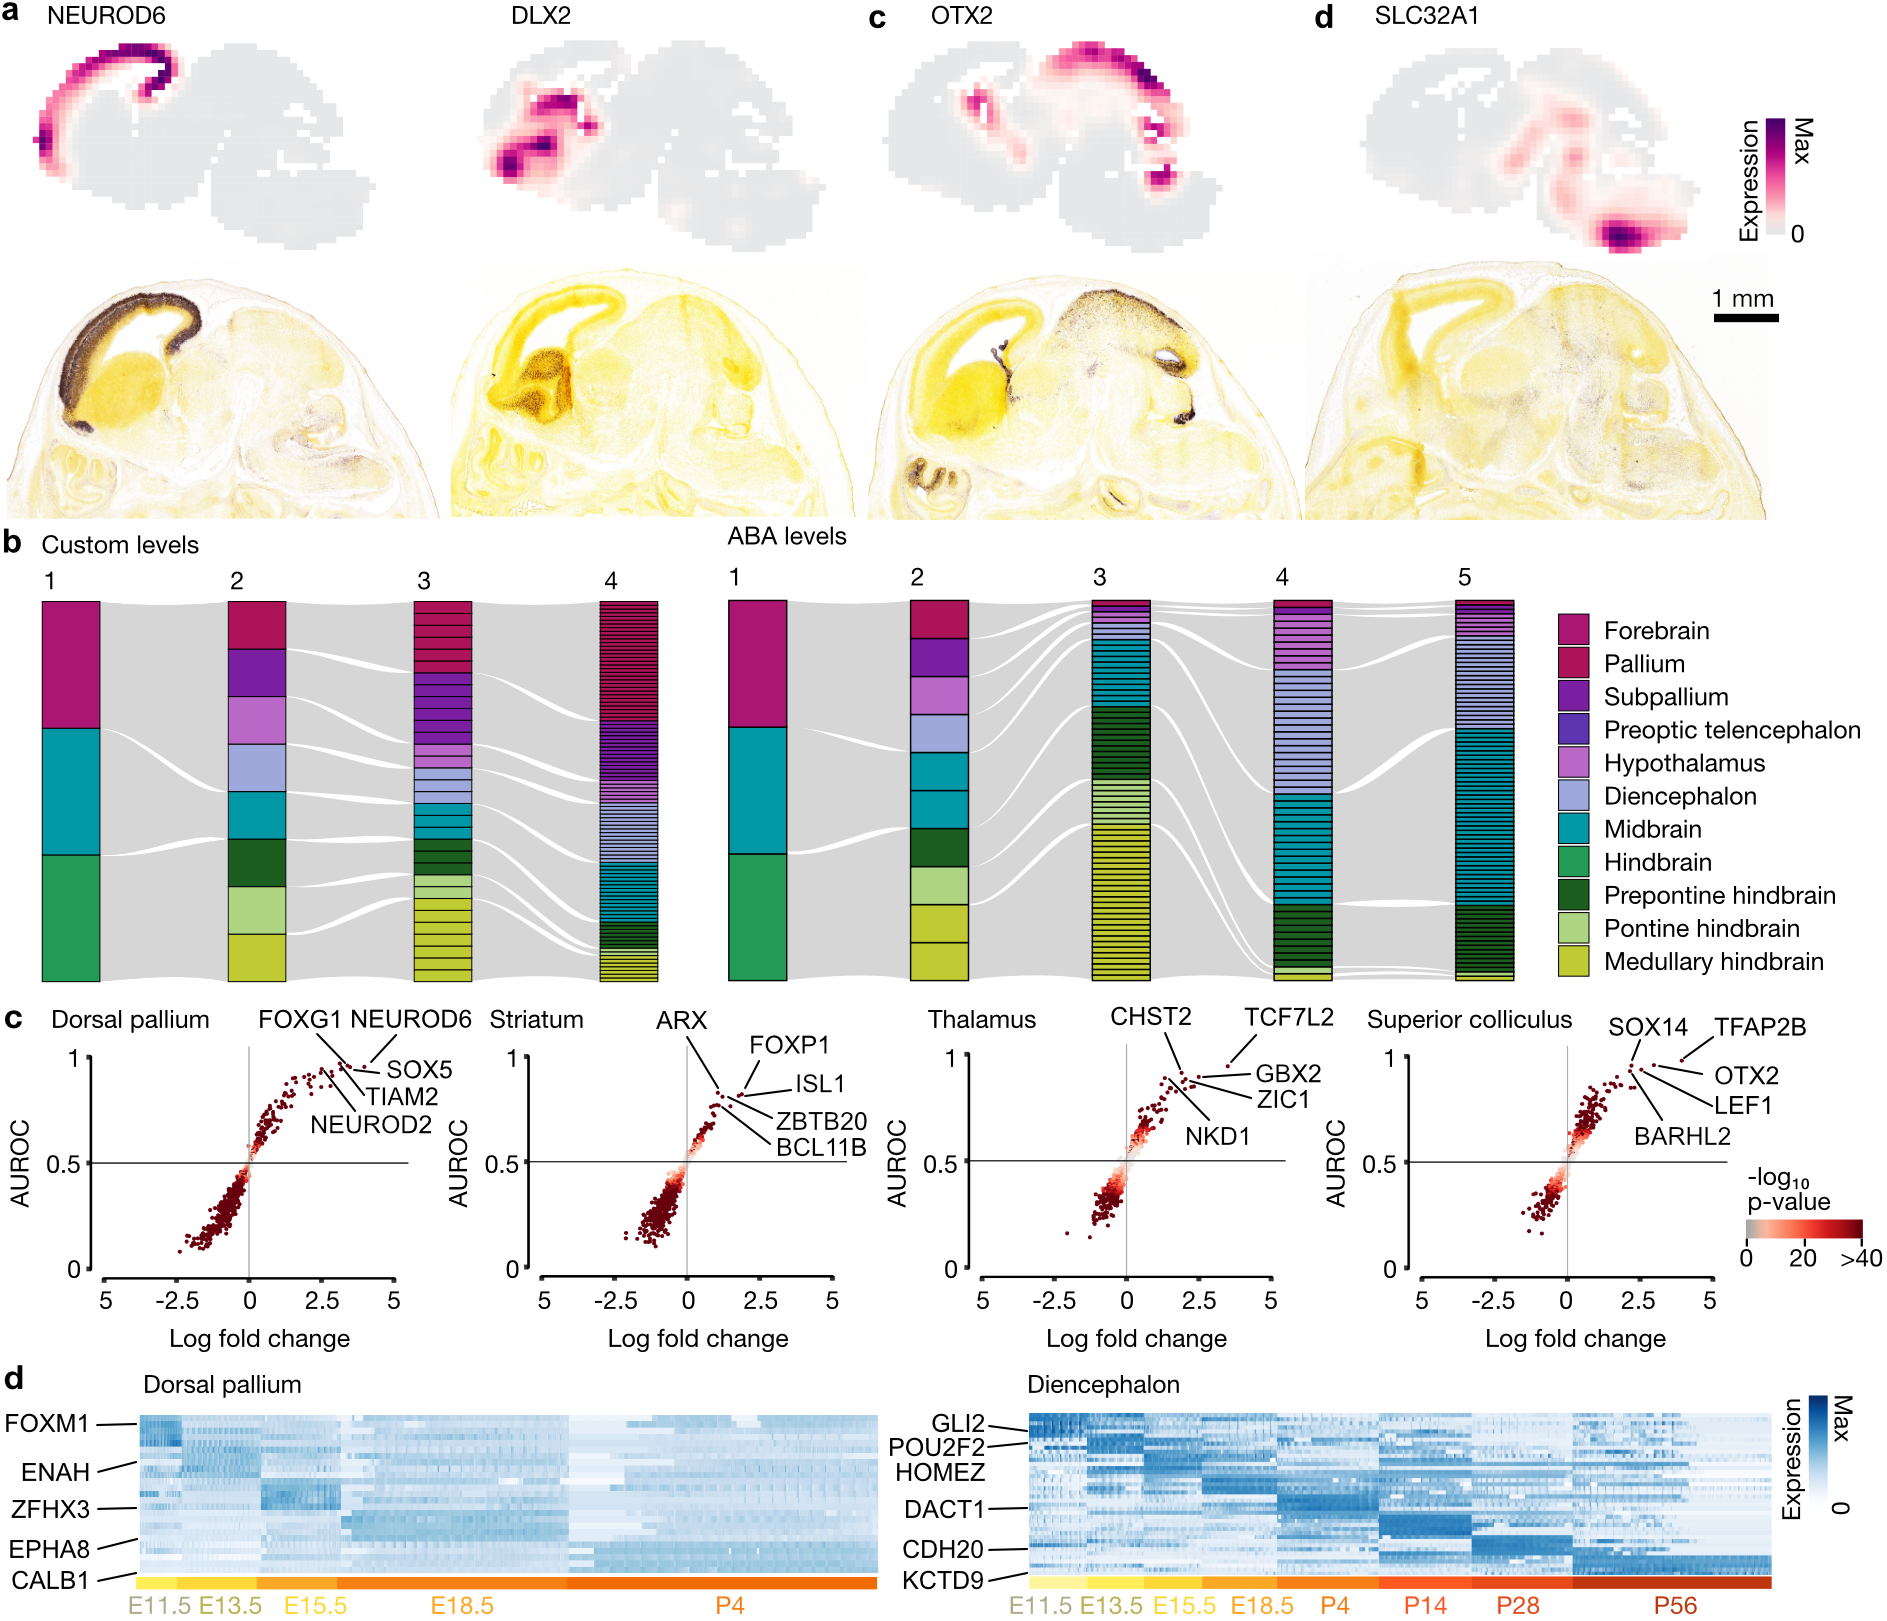
\includegraphics[width=\textwidth]{figures/voxhunt/Supp_1}
    \caption{\textbf{Supplemental characterization of voxel maps of developing mouse brain in situ hybridization data, related to Figure 2.2.} a) In silico expression maps compared to in situ hybridization patterns. Voxelized expression heatmaps (top) and in situ hybridization head images from the Allen Developing Mouse Brain Atlas (bottom) at E15.5 for NEUROD6, DLX2, OTX2, and SLC32A1. b) Hierarchical annotation levels of the developing mouse brain. Barcharts show how large structures are hierarchically subdivided into many smaller structures for custom annotation levels of similar size (left) in comparison to the first five annotation levels from the Allen Brain Atlas (right). Each box represents one annotated structure, colors represent custom level 1 on the first level and custom level 2 on all subsequent levels. c) Scatter plot showing feature selection for dorsal pallium, striatum, thalamus and superior colliculus. X-axis represents fold change and y-axis represents the area under the receiver operating characteristic curve (AUROC) metric for comparisons between the selected structure and all other brain structures. d) Heatmaps showing stage-specific genes for dorsal pallium and diencephalon binned by expression in the corresponding brain structure at different timepoints during development.}
    \label{fig:voxS1}
\end{figure}

\begin{figure}[h!]
    \centering
	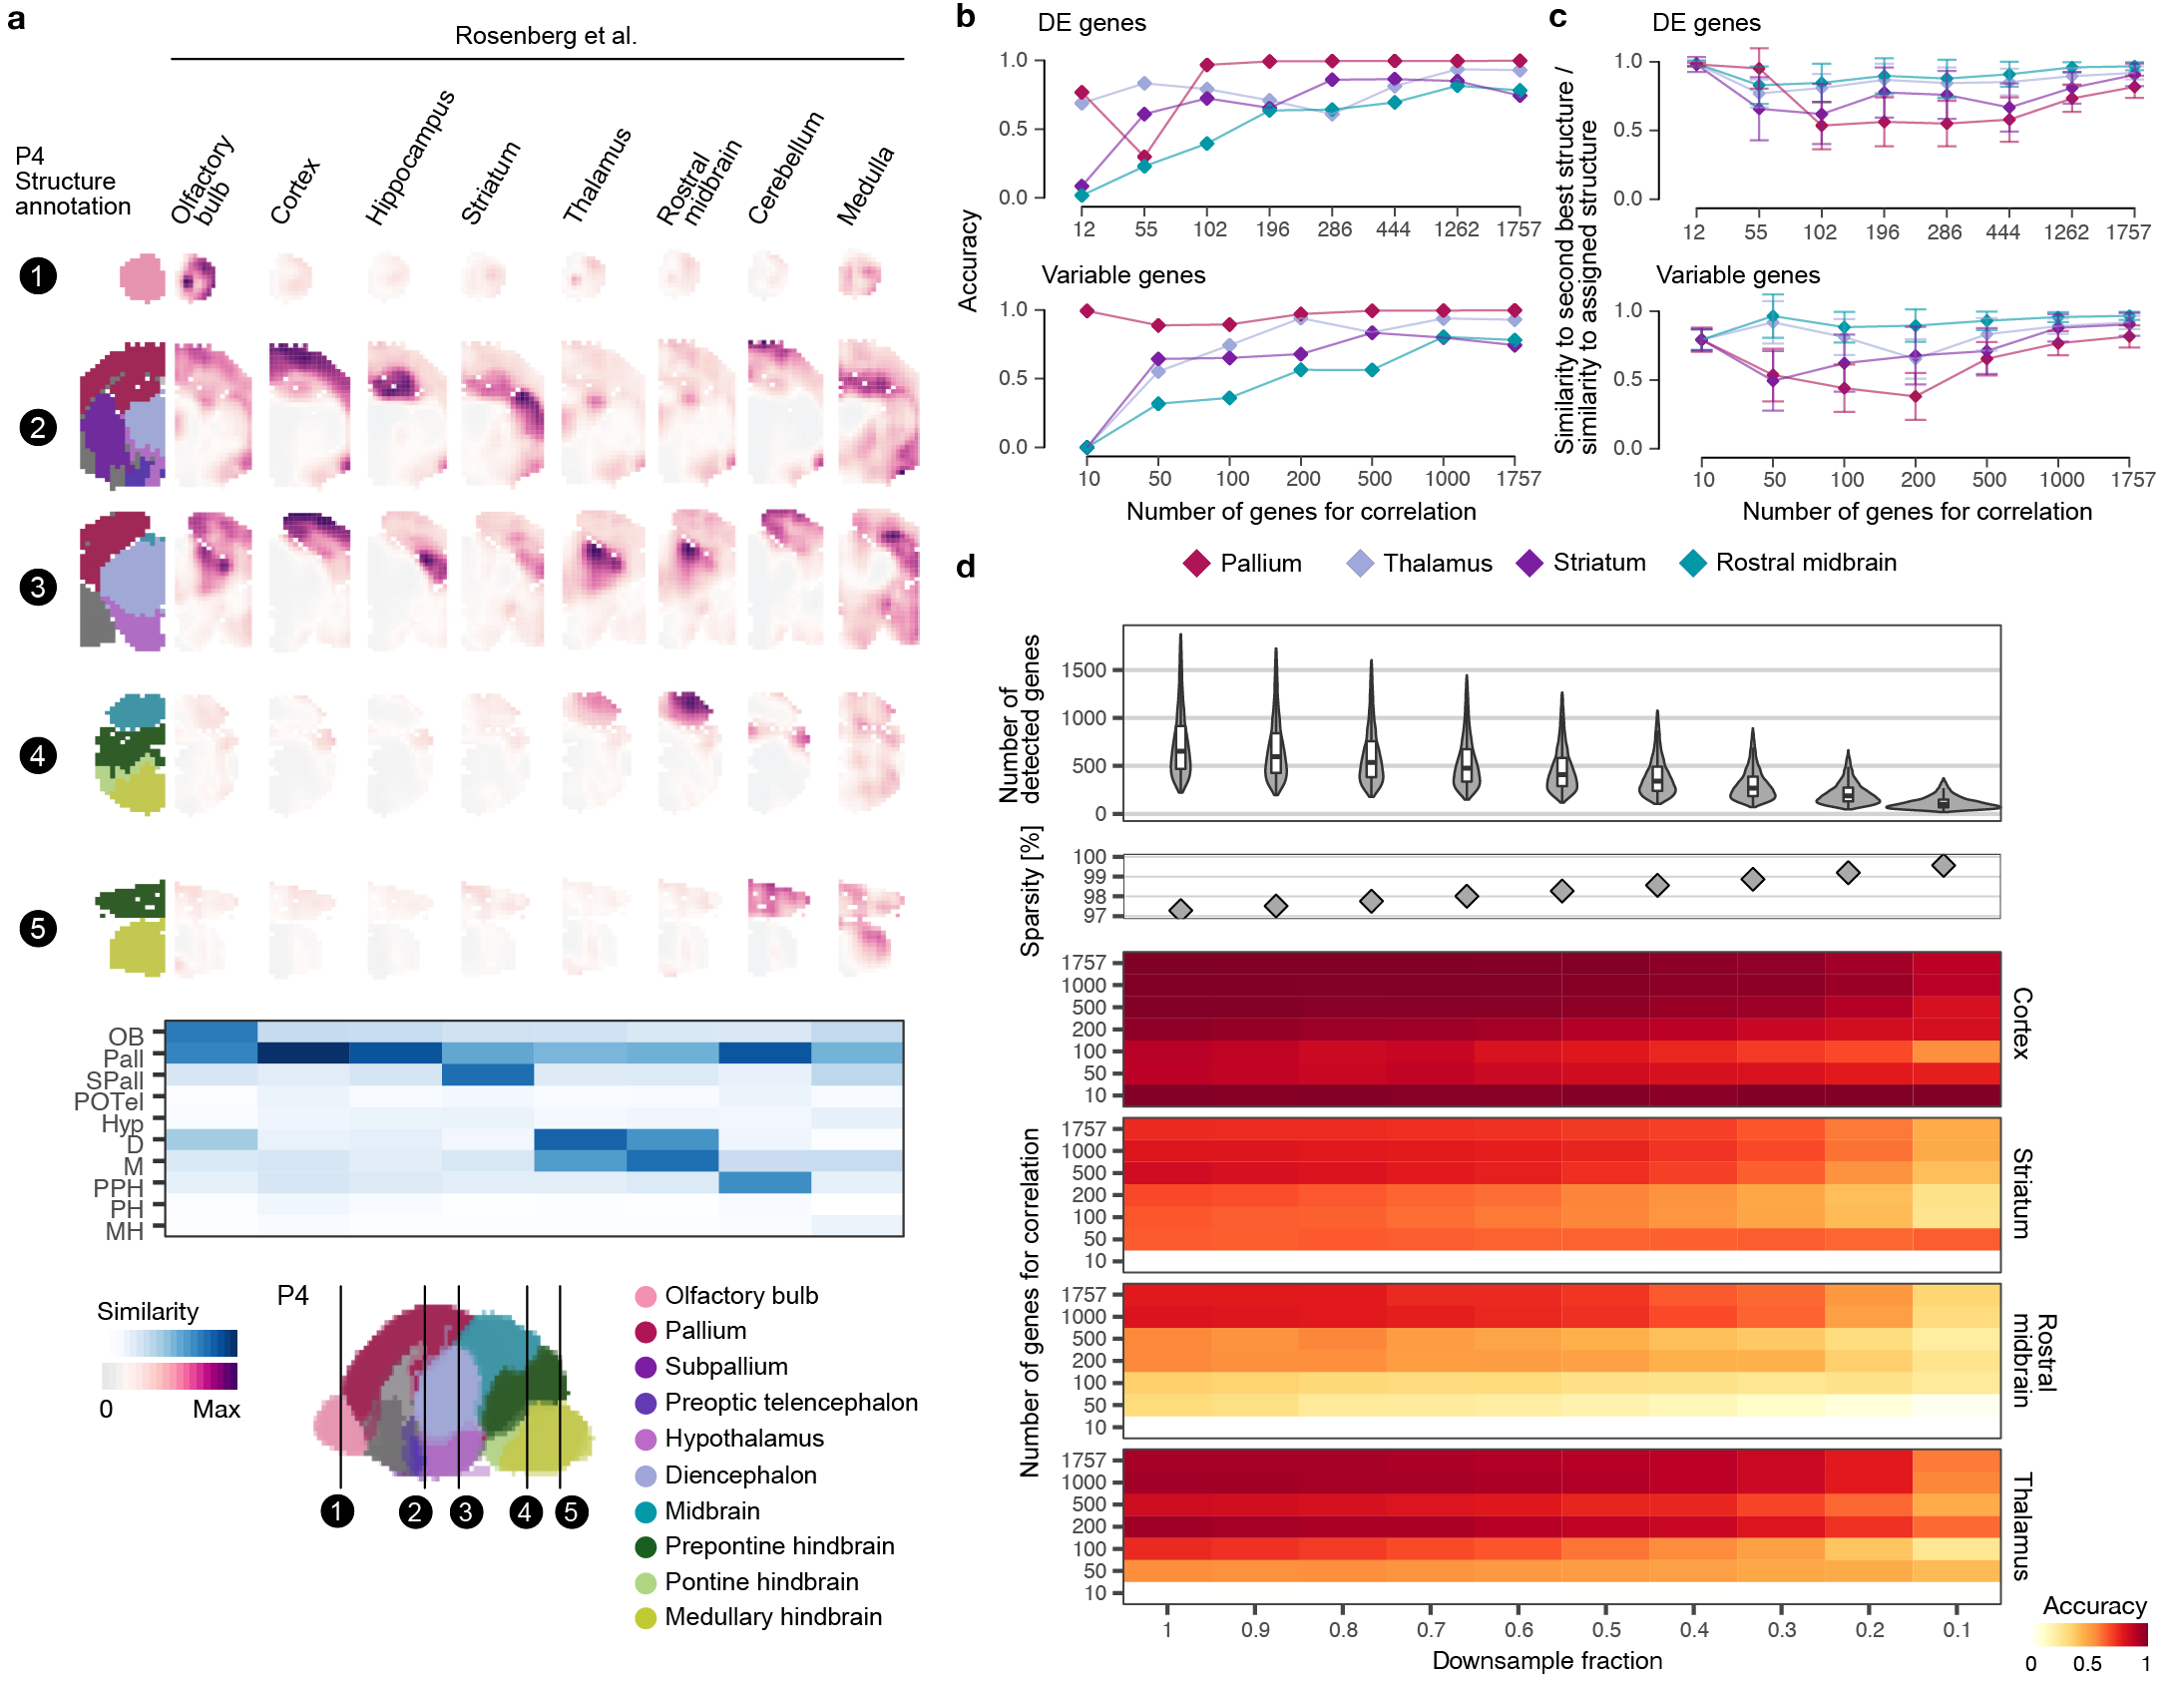
\includegraphics[width=\textwidth]{figures/voxhunt/Supp_2}
    \caption{\textbf{Effect of feature sets and data quality on spatial mapping, related to Figure 2.3.} a) Top: Coronal sections visualizing regional annotation and similarity of different neuronal populations from scRNA-seq of the P2 mouse brain (Rosenberg et al., 2018) to voxel maps of the P4 mouse brain. Bottom: Heatmap visualizing the mean similarity of these neuronal populations to brain structures at custom annotation level 2. b-d) Neuronal populations from scRNA-seq of the P2 mouse brain (Rosenberg et al., 2018) were used to assess accuracy and contrast of the spatial mapping to the P4 mouse brain under different conditions. b) Accuracy of maximum-similarity structure assignments using different numbers of features and feature selection criteria. We either considered the top differentially expressed genes between brain structures (top) or the most variable features (bottom). c) Contrast of spatial brain maps as determined by the ratio of correlation between the two most similar brain structures. Low values indicate high contrast. d) Stability of structure assignments to lower data quality assessed through downsampling of UMI counts. Top: Boxplots showing the number of detected genes per cell for different downsampling fractions. Middle: Fraction of zero entries in the expression matrix for different downsampling fractions. Bottom: Heatmaps showing the accuracy of structure assignments of four neuronal cell populations for different downsampling fractions and feature sets.}
    \label{fig:voxS2}
\end{figure}

\begin{figure}[h!]
    \centering
	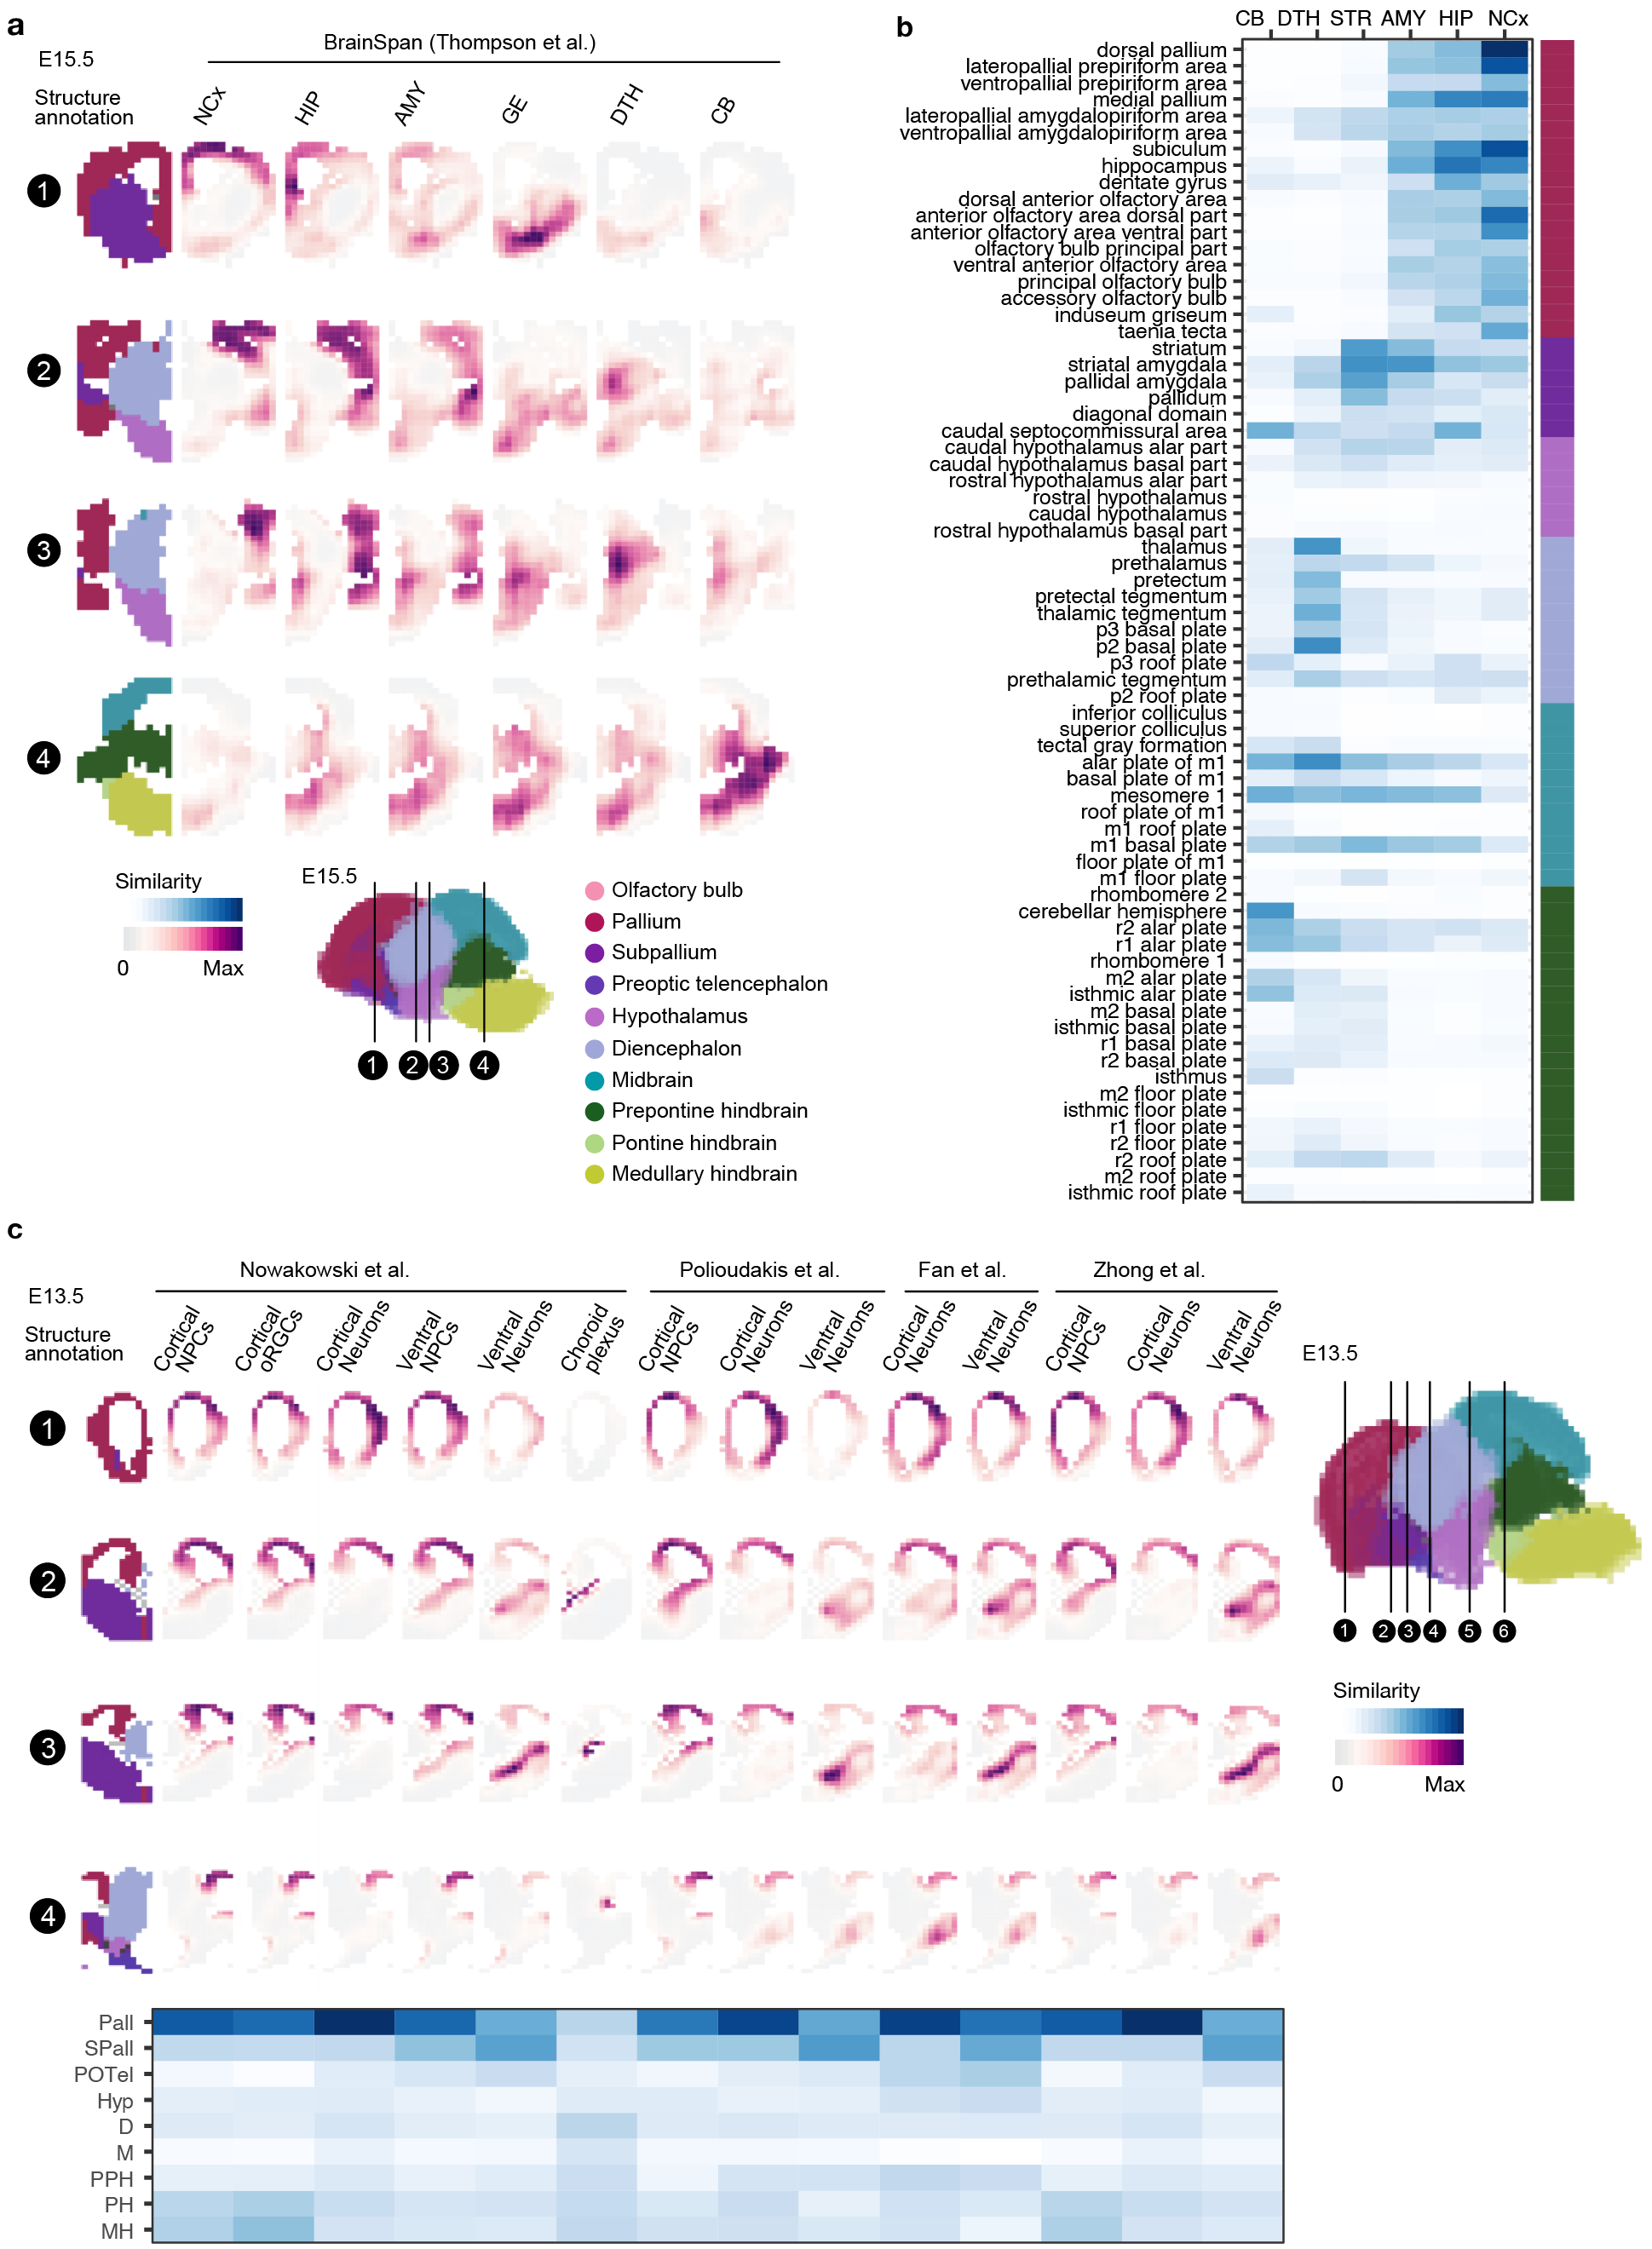
\includegraphics[width=\textwidth]{figures/voxhunt/Supp_3}
    \label{fig:voxS3}
\end{figure}

\begin{figure}[t!]
    \centering
    \caption{\textbf{Spatial similarity maps of brain regions and neuronal cells from primary human tissues, related to Figure 2.3.} a) Coronal sections visualizing regional annotation and scaled similarity scores of bulk RNA-seq data from microdissected human brain structures (wpc12 - wpc20) from BrainSpan to voxel maps of the E15.5 mouse brain. b) Heatmap showing similarity of microdissected human brain structures to E13.5 mouse brain structures at custom annotation level 4. c) Top: Coronal sections visualizing regional annotation and scaled similarity scores of human neuronal cell types from different studies to voxel maps of the E13.5 mouse brain. Bottom: Heatmap visualizing the mean similarity of neuronal cell populations to structures in the E13.5 mouse brain. NCx: neocortex, HIP: hippocampus, AMY: amygdala, GE: ganglionic eminence, DTH: dorsal thalamus, CB: cerebellum. NPC: Neural progenitor cell, oRGs: outer radial glia cells.}
\end{figure}


\begin{figure}[h!]
    \centering
	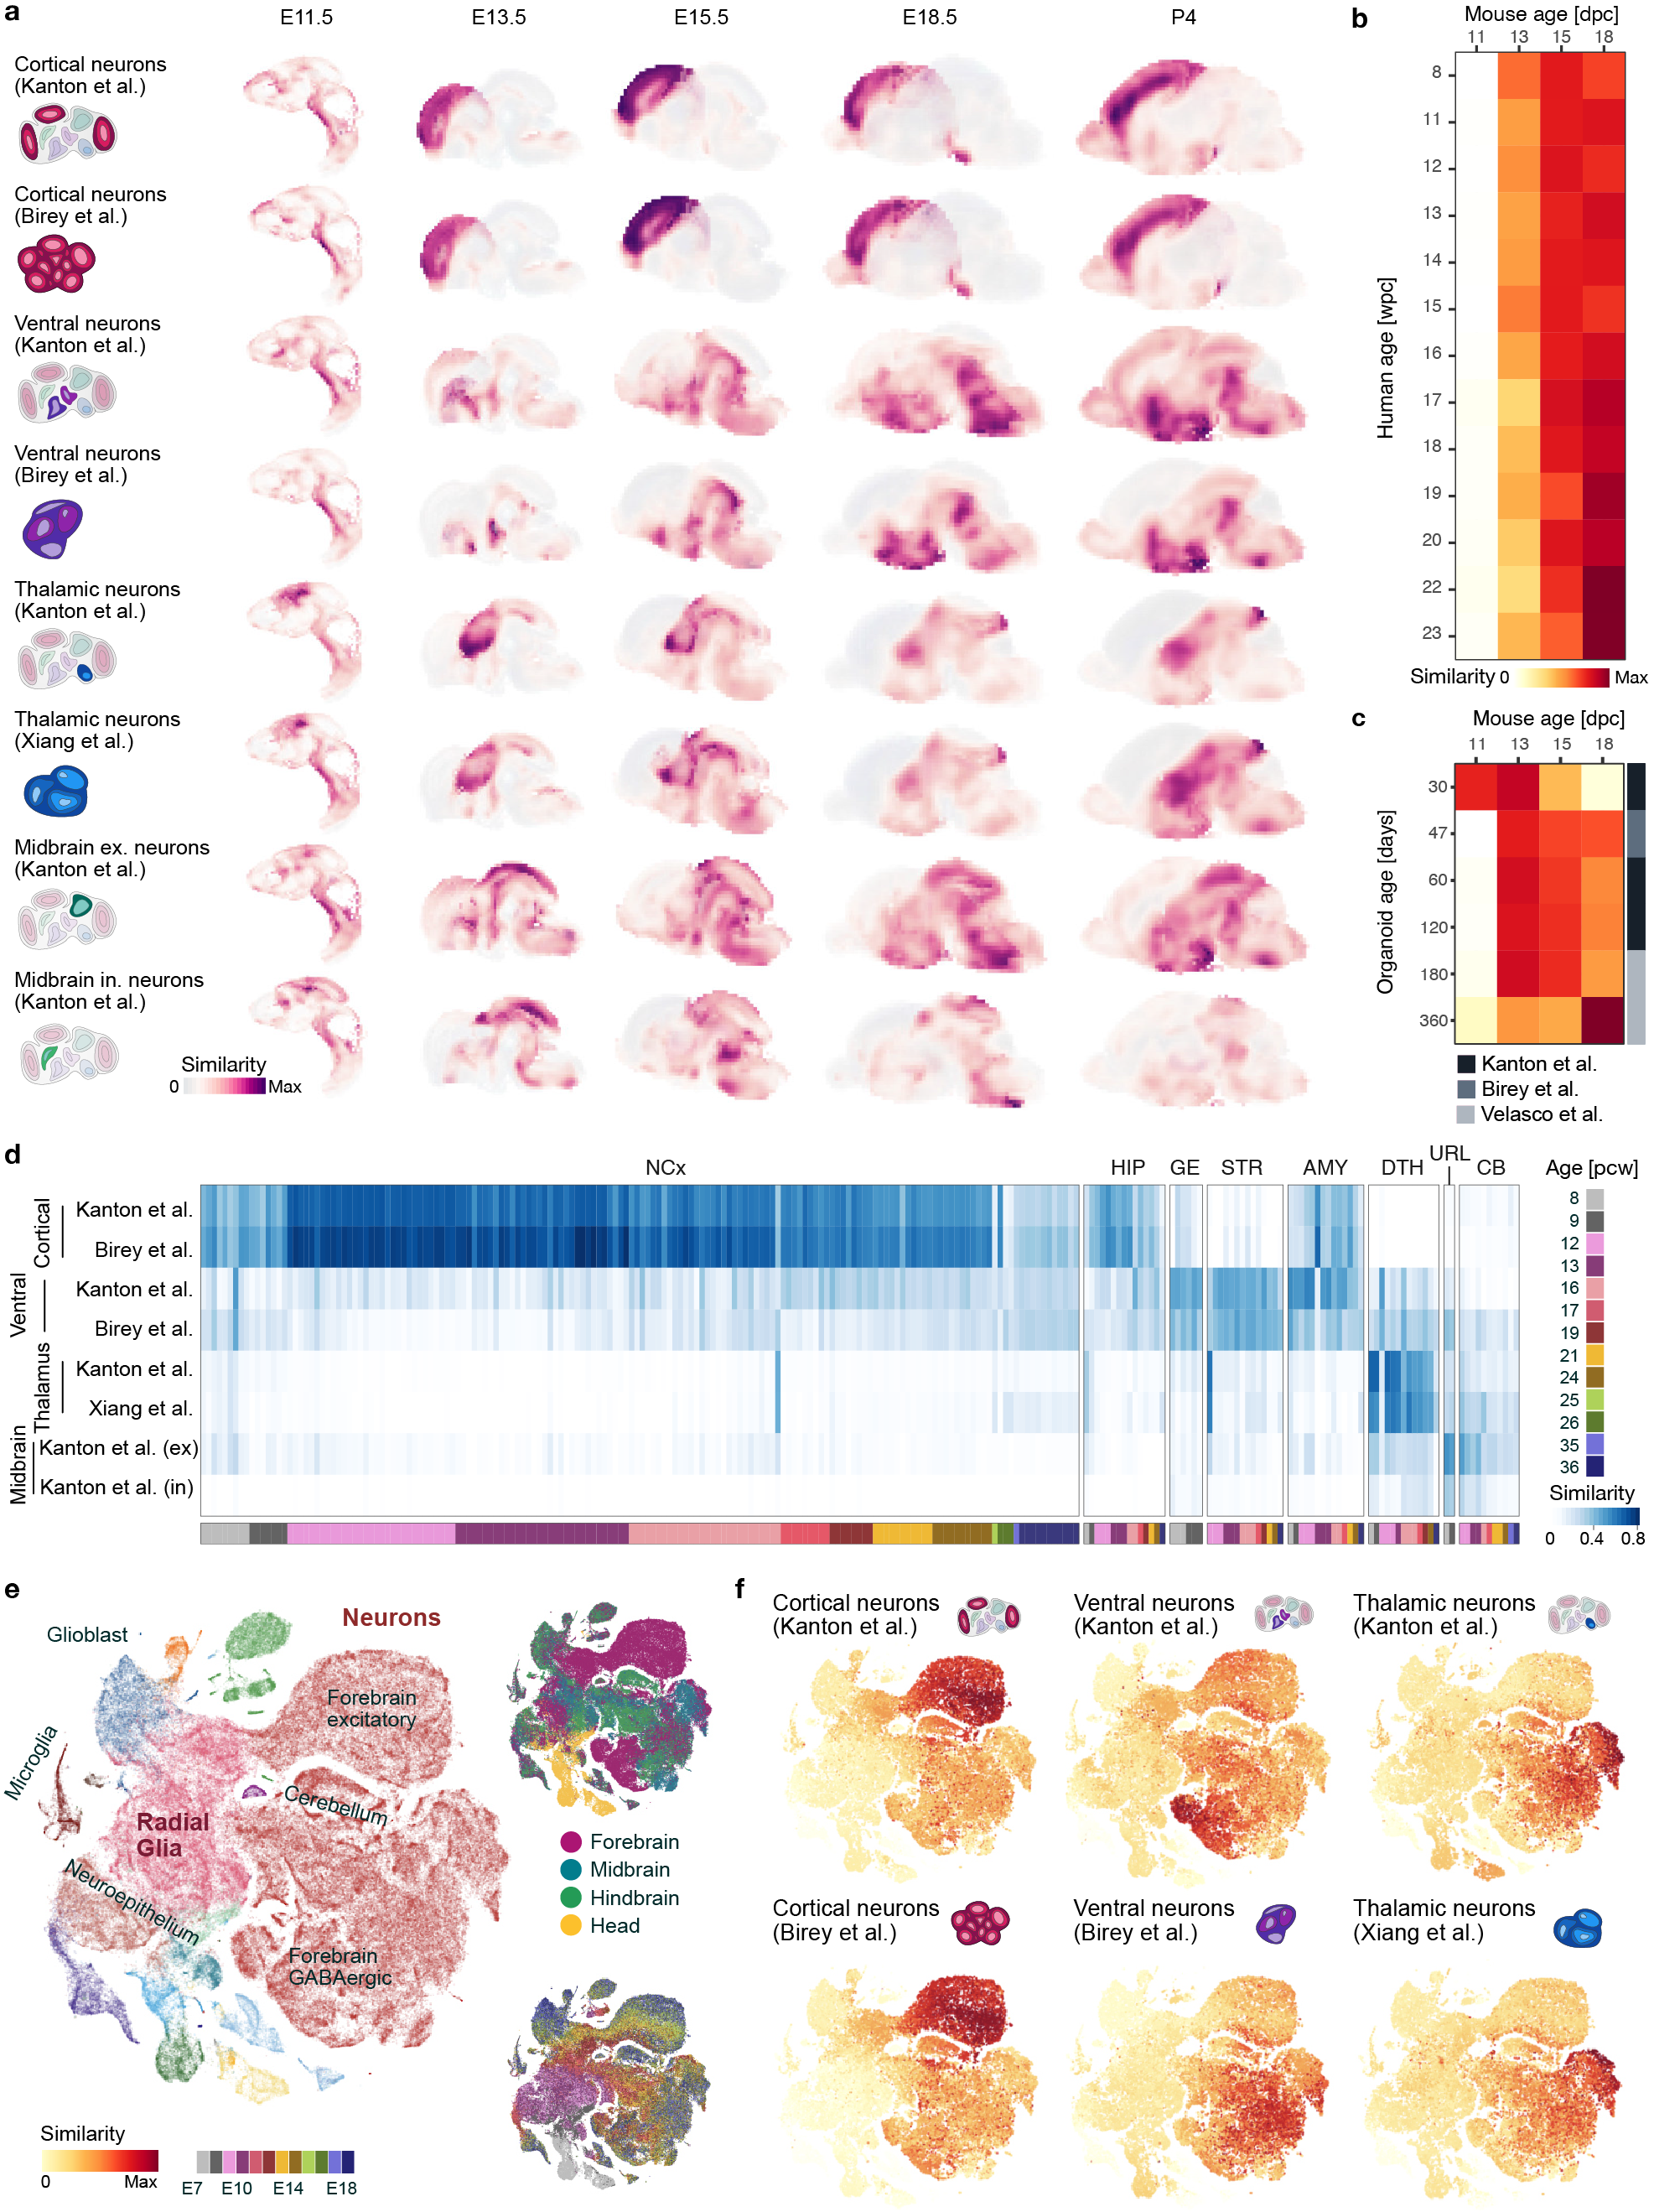
\includegraphics[width=\textwidth]{figures/voxhunt/Supp_4}
    \label{fig:voxS4}
\end{figure}

\begin{figure}[h!]
    \centering
    \caption{\textbf{Comparing brain organoid cell populations to reference brain maps, related to Figure 2.4.} a) Sagittal projections colored by scaled similarity scores of different organoid clusters from each organoid dataset to voxel maps of the developing mouse brain in stages E11.5 - P4. b) Heatmap showing the similarity of cortical neurons across human fetal development to the developing mouse pallium 11 - 18 dpc. For each population of cortical neurons and mouse developmental stage, we computed the mean of maximum correlating voxels in the mouse pallium. c) Similarity of cortical neurons from organoids grown through three different protocols (Birey et al., 2017; Kanton et al., 2019; Velasco et al., 2019) at 30 - 360 days of age to the mouse pallium at 11 - 18 dpc. d) Heatmap showing the similarity of organoid cell populations to bulk transcriptomes of microdissected human brain structures from BrainSpan. e) Structure, cell type and age annotations for the developing mouse brain dataset. NPC: Neural progenitor cell, CBC: Cilia bearing cell, ChP: Choroid plexus, Pall: Pallium, Spall: Subpallium, PPH: Prepontine hindbrain, NCx: Neocortex, HIP: Hippocampus, GE: Ganglionic eminence, STR: Striatum, AMY: Amygdala, DTH: Dorsal thalamus, URL: Upper rhombic lip, CB: Cerebellum. f) Scaled similarity scores of organoid cell populations to single cell transcriptomic data of the developing mouse brain (La Manno et al., 2020).}
\end{figure}

\begin{figure}[h!]
    \centering
	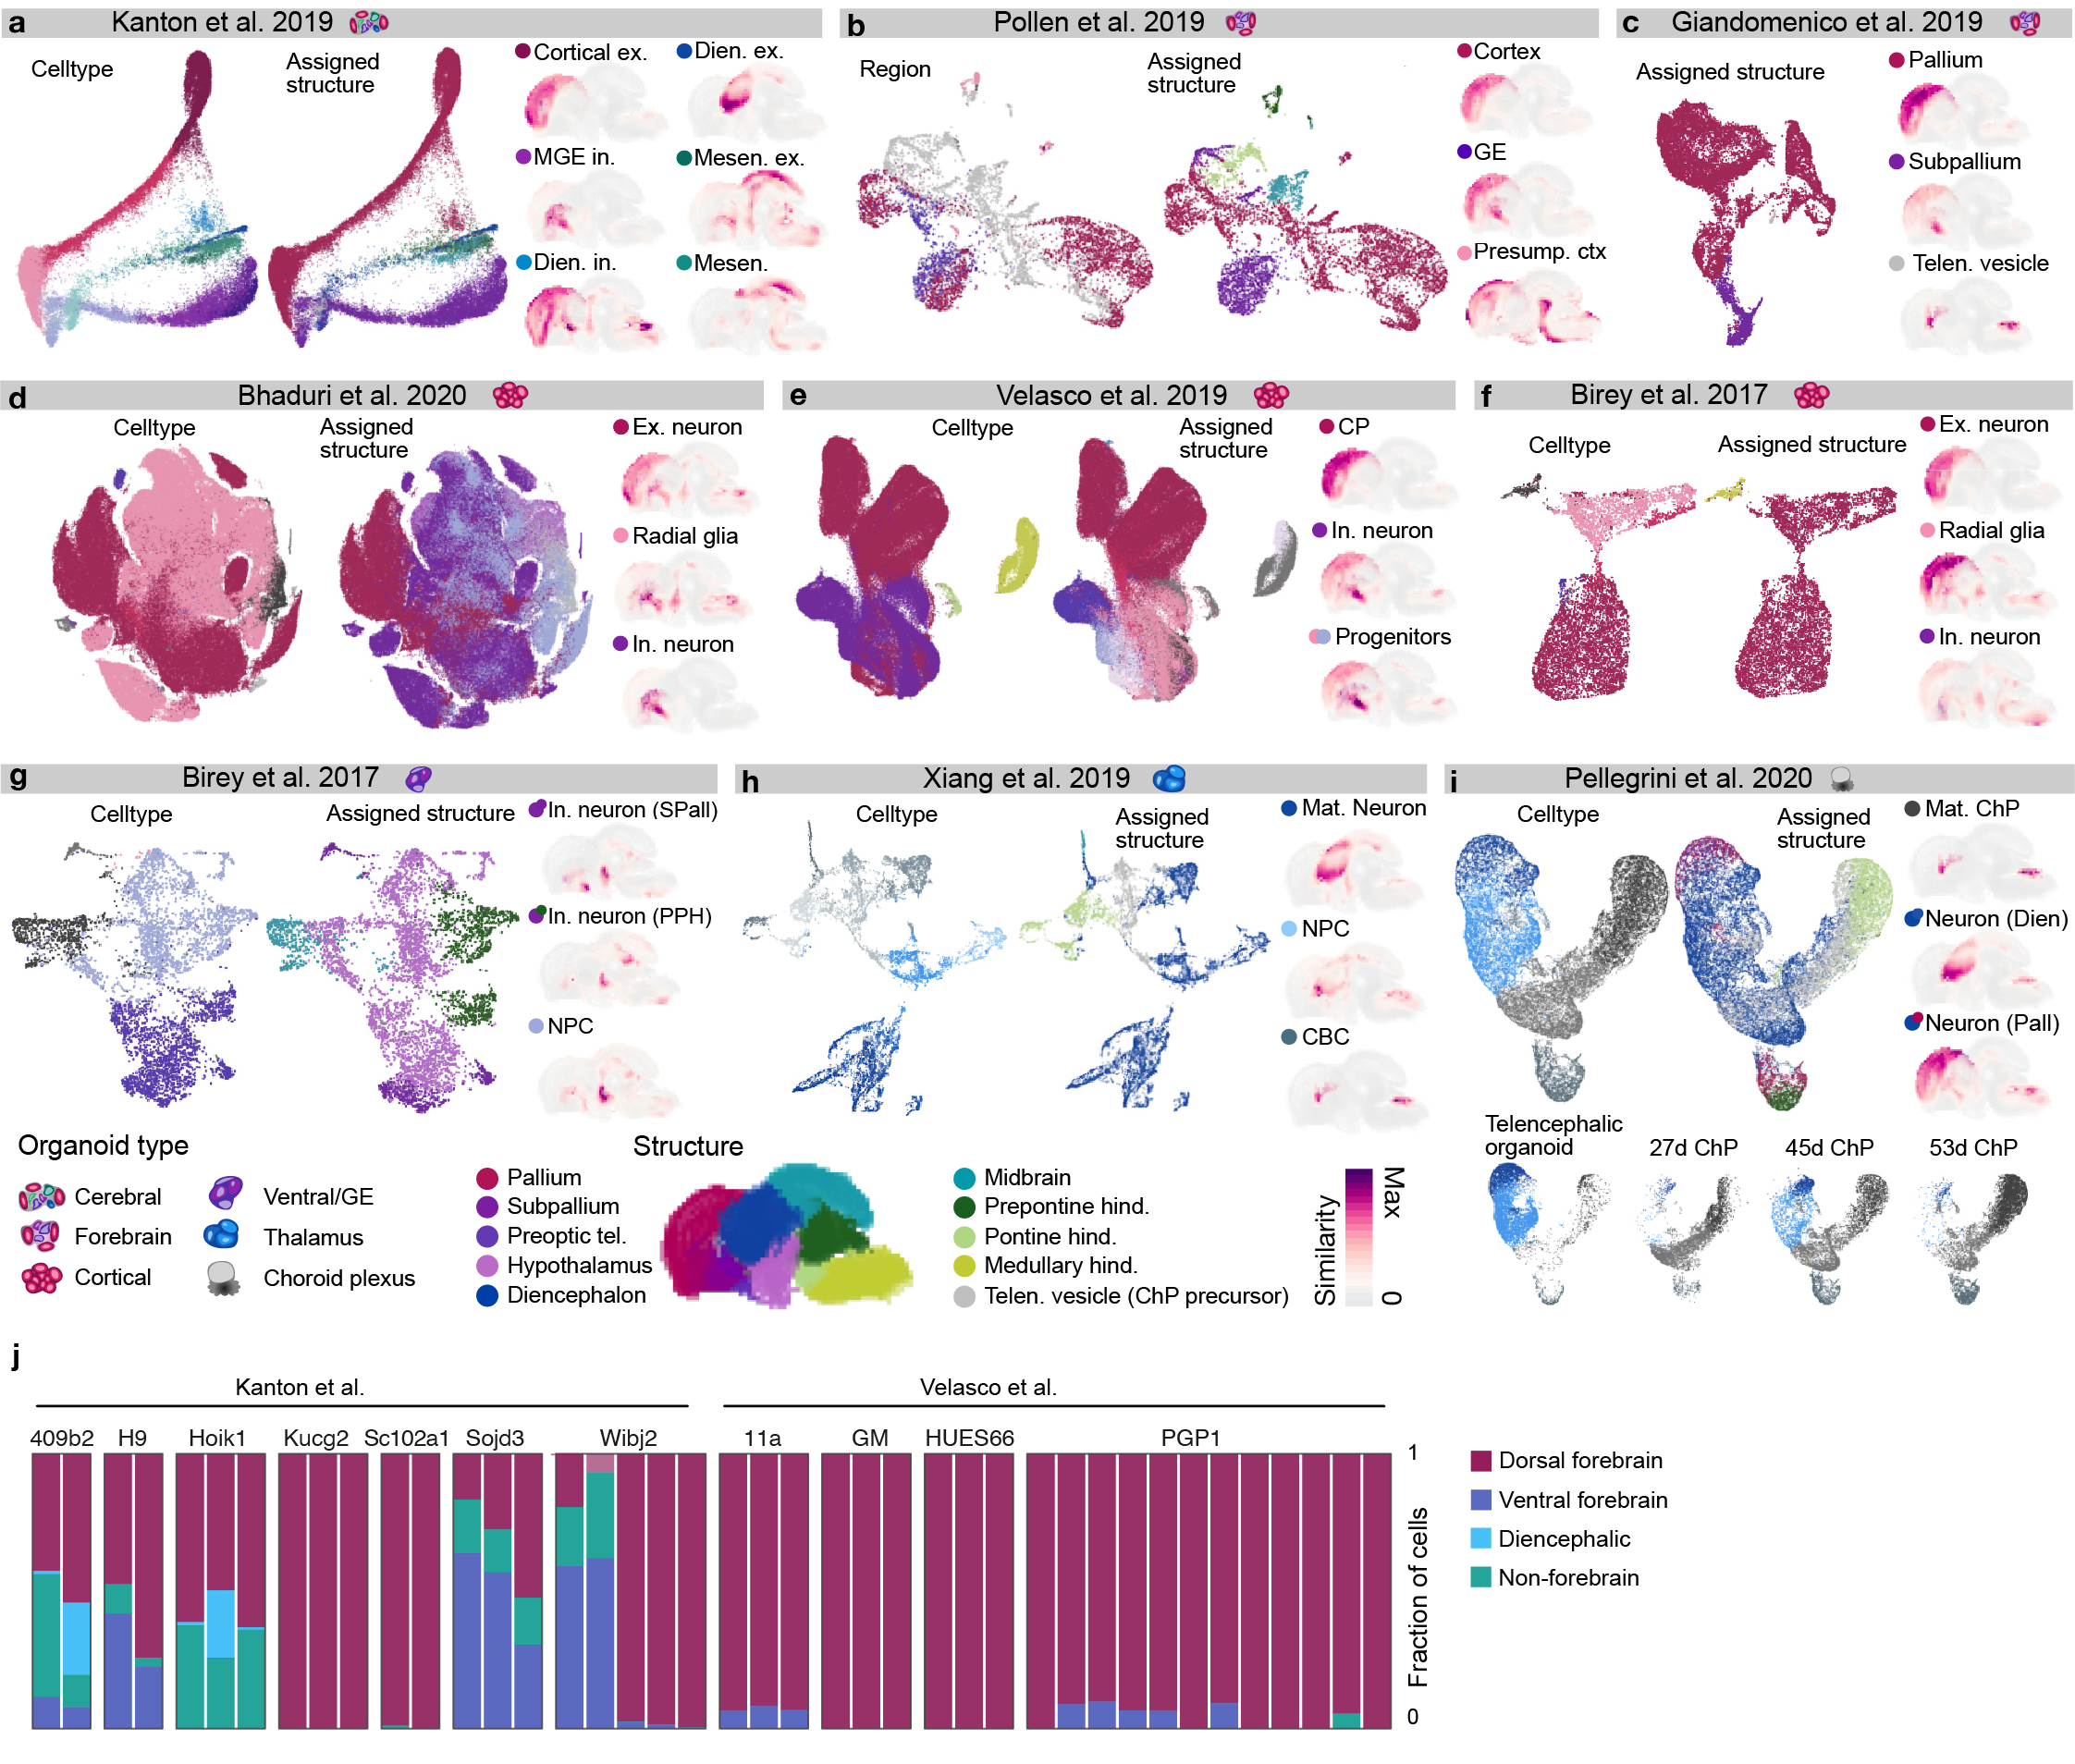
\includegraphics[width=\textwidth]{figures/voxhunt/Supp_5}
    \caption{\textbf{Comparing cell populations from different organoid protocols to spatial brain maps, related to Figure 2.4.} a-i) Brain region identities of organoid cell types from various published datasets. Cells are plotted using the embedding coordinates from the original publication (where available) or a custom UMAP embedding. For each dataset, the left panel shows cells colored by region or cell type where annotations were publicly available. The middle panel shows the clusters of cells colored by the brain structure containing the most highly correlated voxel of the average cluster transcriptome. The right panel shows sagittal sections visualizing scaled similarity scores of organoid cell populations to voxel transcriptomes. j) Comparison of organoids from different stem cell lines and batches with regard to their composition of neuron populations as annotated by VoxHunt. Each stacked bar plot represents scRNA-seq data from a single organoid.}
    \label{fig:voxS5}
\end{figure}

\begin{figure}[h!]
    \centering
	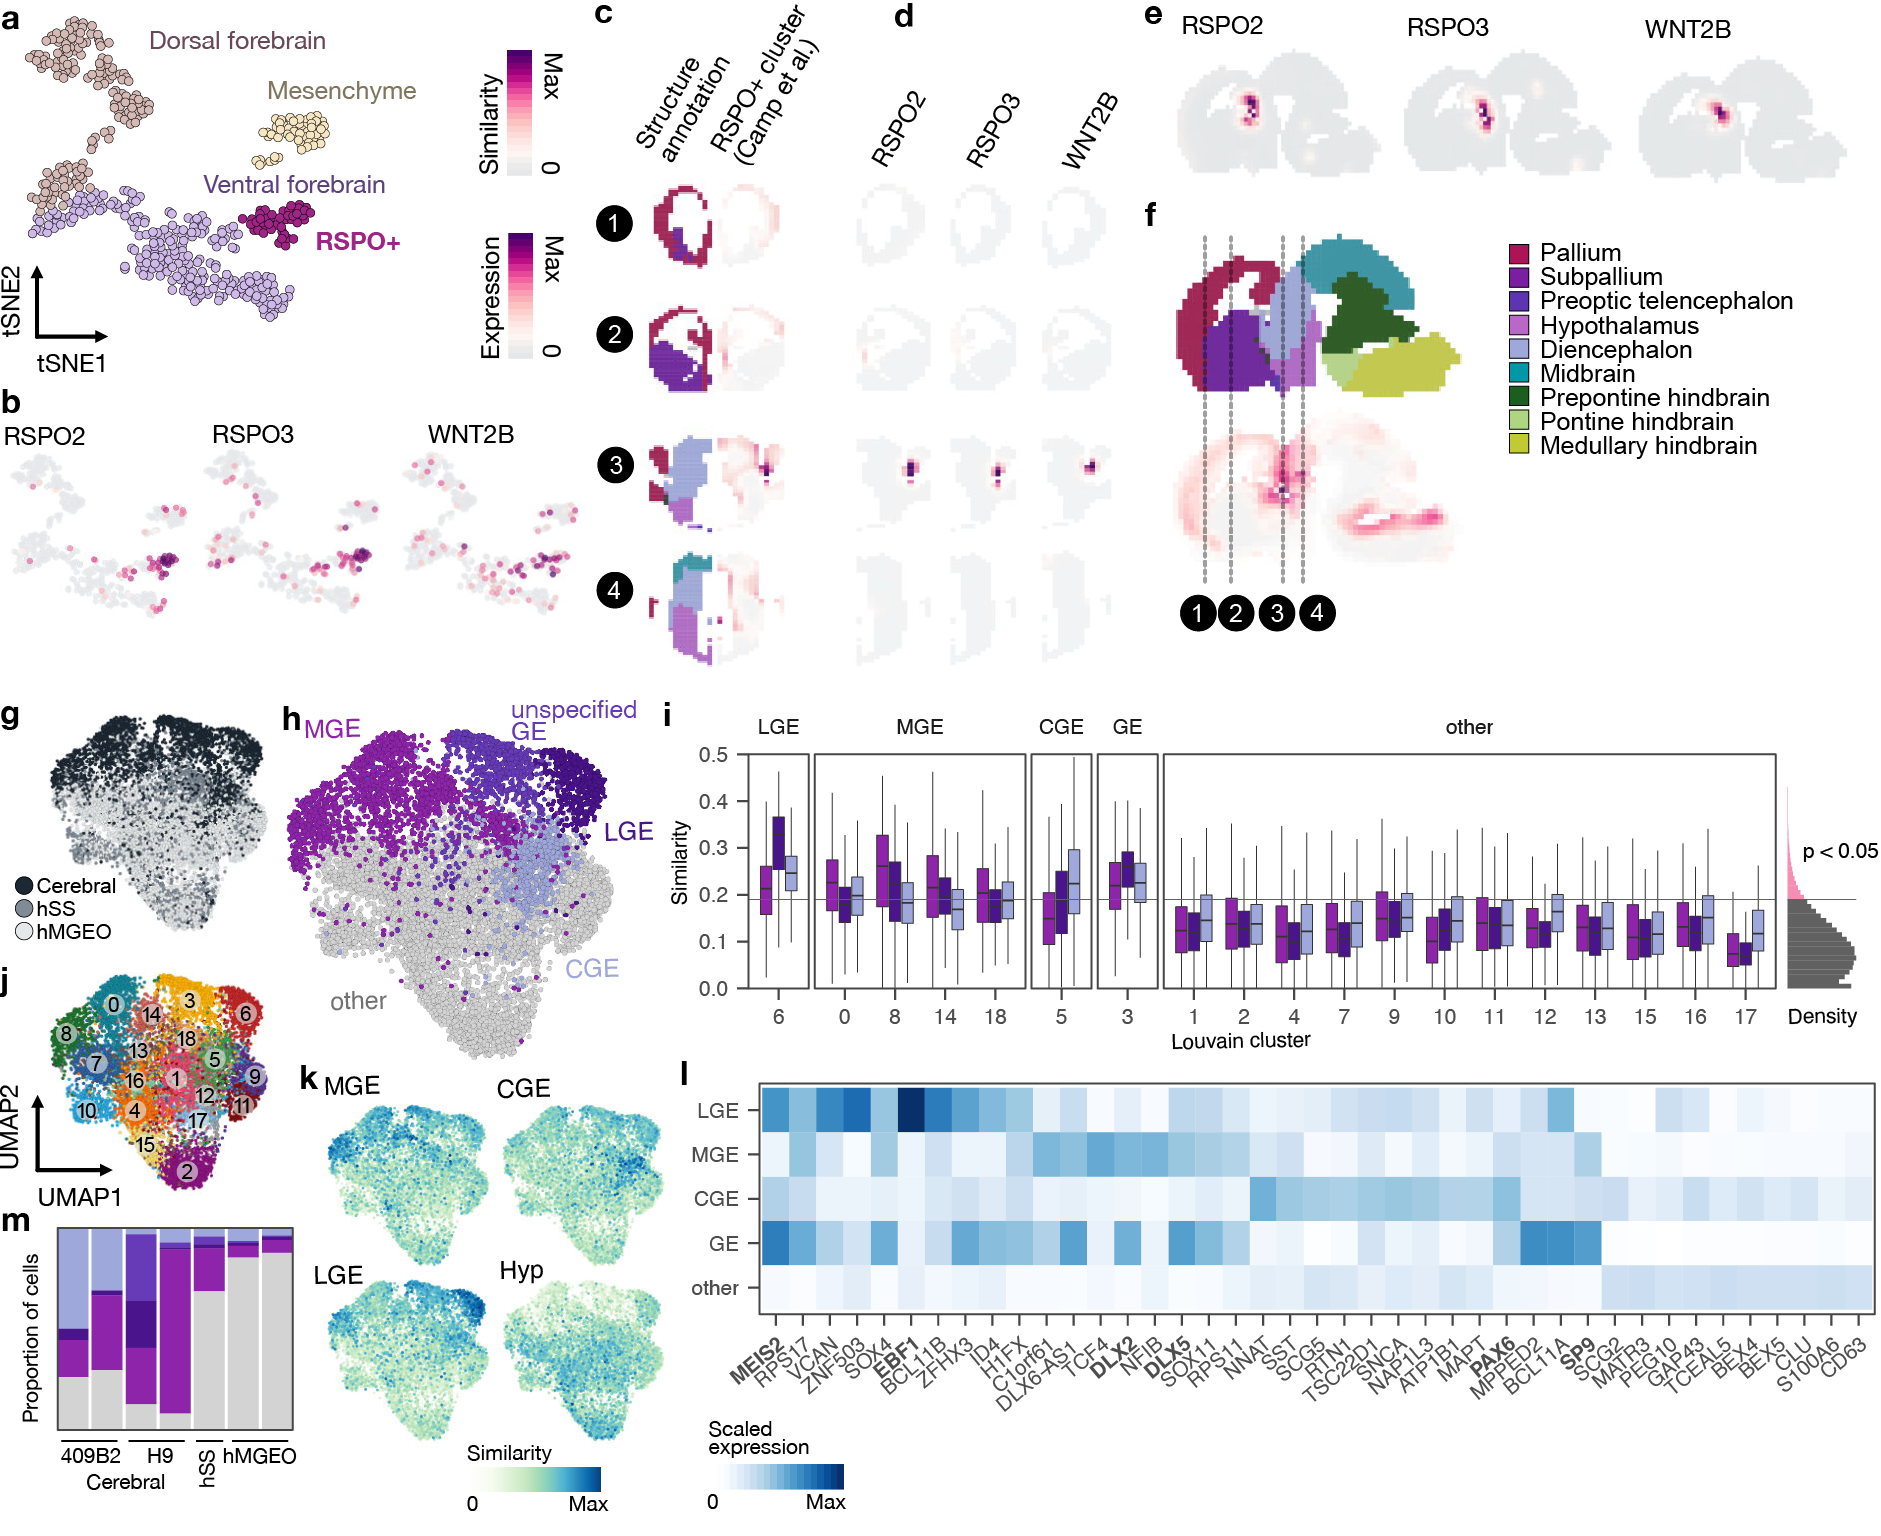
\includegraphics[width=\textwidth]{figures/voxhunt/Supp_6}
    \caption{\textbf{Spatial similarity maps resolve substructure identity of organoid cells, related to Figure 2.5.} a) tSNE embedding of single-cell transcriptomes from cerebral organoid cells based on the SMART-SEQ protocol implemented using Fluidigm C1 (Camp et al., 2015).  The previously unknown ‘RSPO+’ cluster is highlighted in purple. b) tSNE embedding colored by expression of genes marking the ‘RSPO+’ cluster. c) Coronal sections (6, 11, 22, 26) visualizing structure annotation and scaled similarity scores to voxel transcriptomes. d-e) Expression patterns of genes marking the ‘RSPO+’ cluster as maximum intensity projections across coronal sections 6, 11, 22 and 26 (d) and sagittal sections 2-5 (e). f) Top: Structure annotation of sagittal sections 2-5 of the E13.5 mouse brain. Bottom: Sagittal projections colored by scaled similarity scores of the ‘RSPO+’ cluster to voxel maps of the E13.5 mouse brain. g-h) A UMAP embedding of the integrated neuronal populations of ventral organoid datasets colored by g) protocol, h) assigned structure identity j) louvain cluster and k) scaled similarity to LGE, CGE, MGE and hypothalamus (Hyp). i) Similarity of louvain clusters to GE substructures LGE, MGE and CGE and distribution of similarity values across all cells. l) Heatmap showing the expression of top marker genes for each neuron population. Canonical GE marker genes are highlighted in bold. m) Neuron composition of individual organoids derived from different protocols (cerebral, hSS and hMGEO) and cell lines (409B2 and H9).}
    \label{fig:voxS6}
\end{figure}

\begin{figure}[h!]
    \centering
	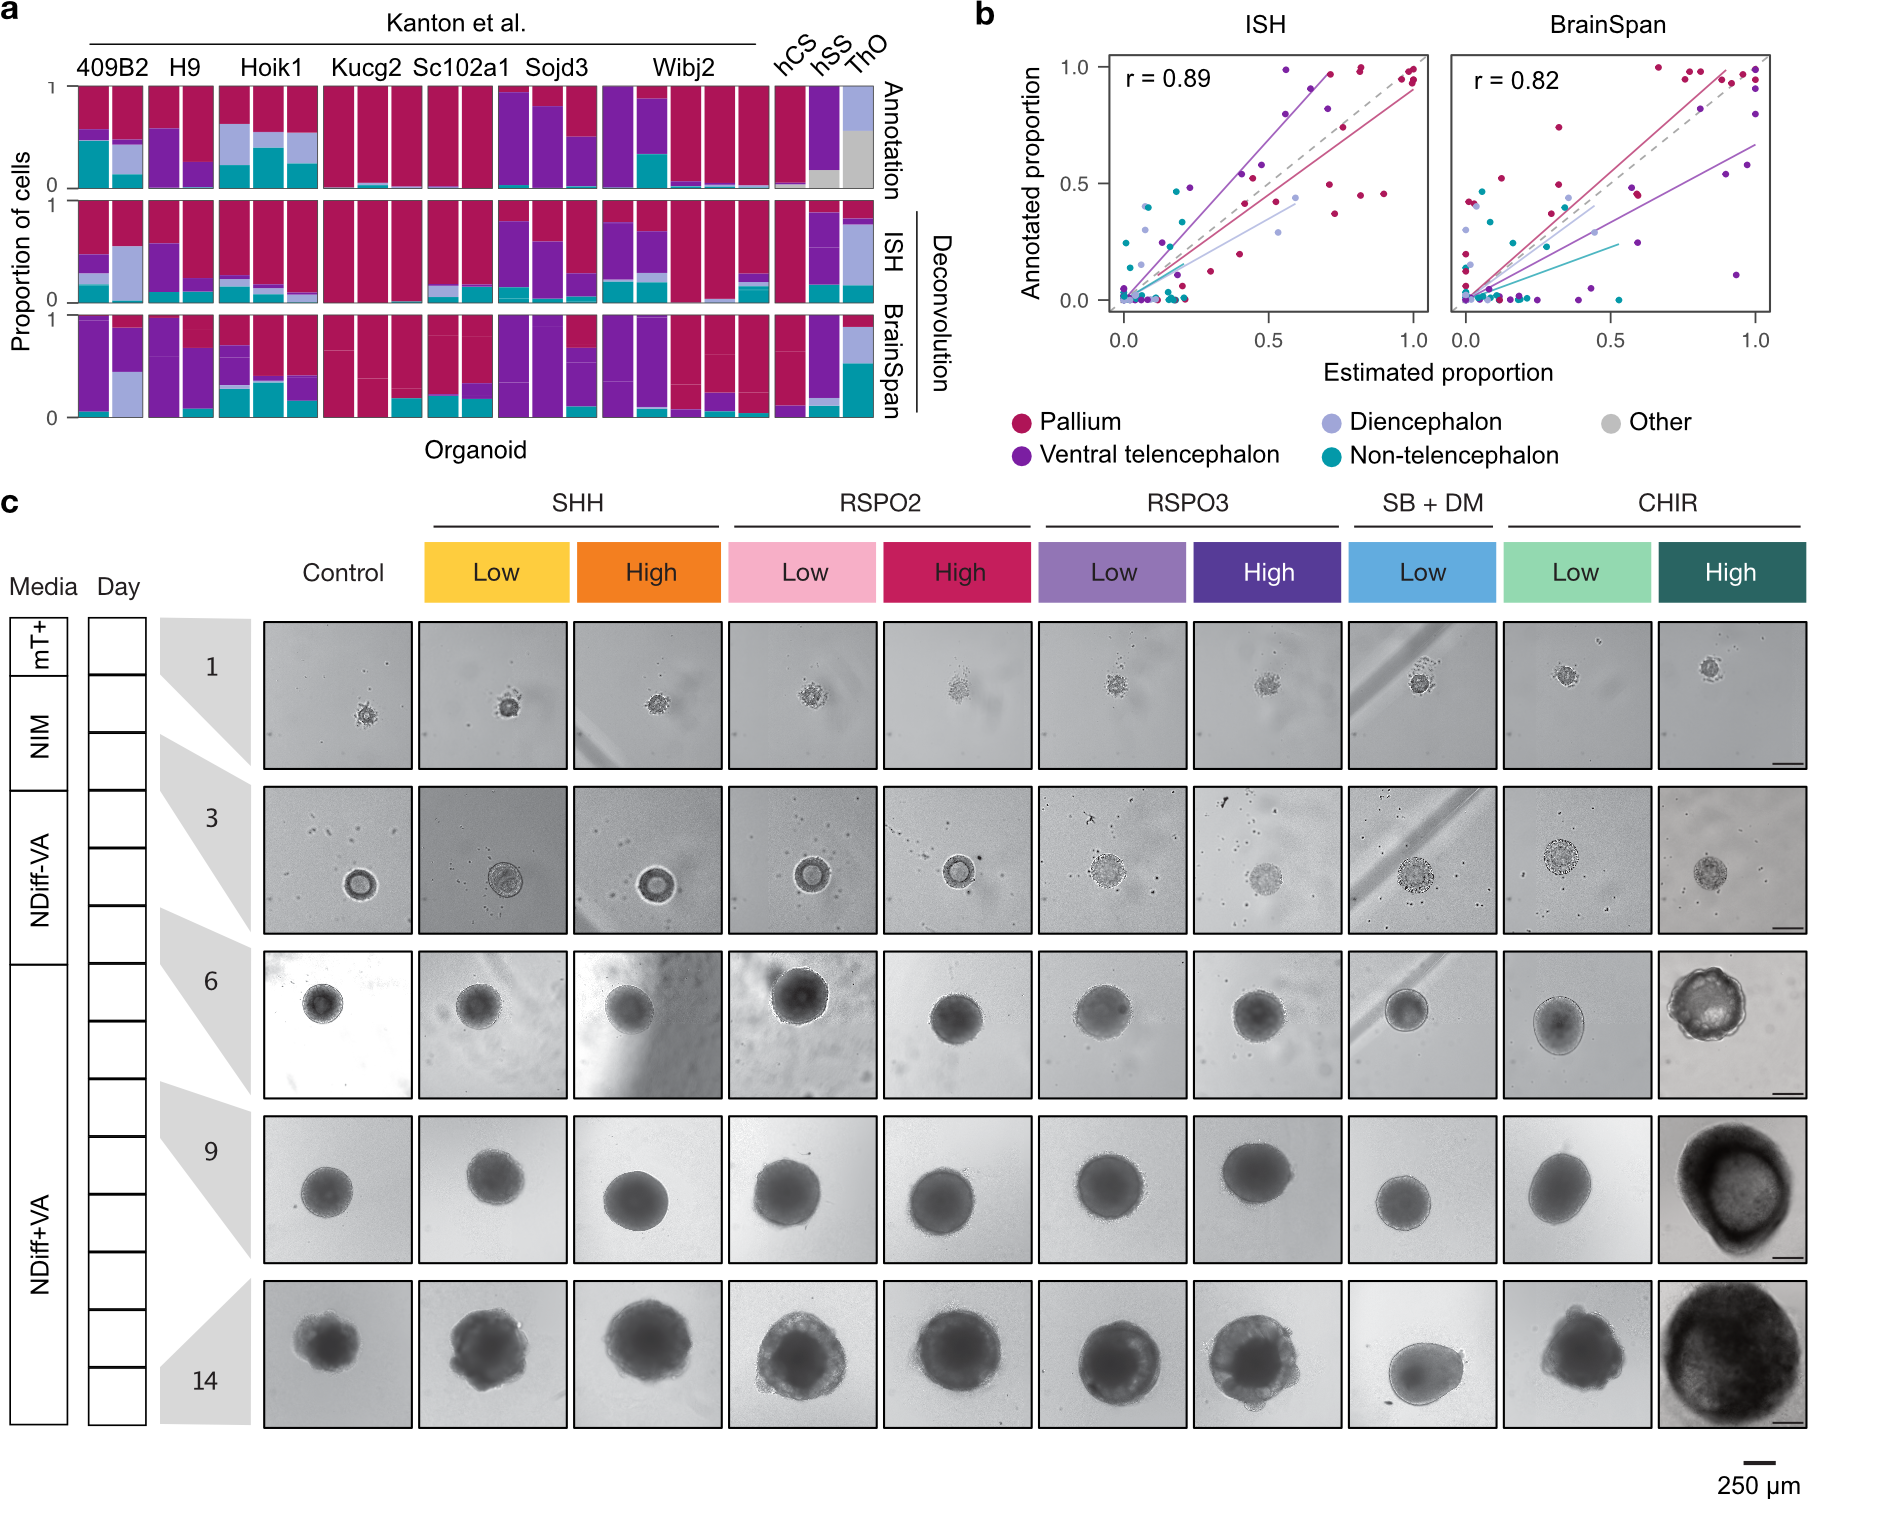
\includegraphics[width=\textwidth]{figures/voxhunt/Supp_7}
    \caption{\textbf{Deconvolution of organoid pseudo-bulk RNA-seq data and images of developing organoids from patterning screen, related to Figure 2.7.} a-b) Single-cell transcriptomics data from different organoid protocols, including cerebral (Kanton et al., 2019), cortical (hCS, (Birey et al., 2017)), ventral (hSS, (Birey et al., 2017)) and thalamic (ThO, (Xiang et al., 2019)) was summarized to pseudo-bulk and deconvoluted using either the Developing Mouse Brain Atlas (ISH) or Brainspan as a reference. a) Proportion of cells in organoids resembling different brain structures as assessed through single-cell transcriptome-based annotations (Annotated) or through deconvolution of pseudo-bulk transcriptomes (Deconvolution). b) Correlation of annotated proportions and proportions estimated through deconvolution. c) Organoids were grown in separate wells of an ultra-low attachment 96-well plate and exposed to different morphogens in low and high doses from day 3 until day 6 of culture. Pictures were taken at regular time points during organoid development.}
    \label{fig:voxS7}
\end{figure}

\clearpage

\topparagraph{Supplementary Data}

\noindent
All supplementary data items can be obtained from polybox with the following link: \\ \href{https://polybox.ethz.ch/index.php/s/FQvxGTwZe6wqNcR}{https://polybox.ethz.ch/index.php/s/FQvxGTwZe6wqNcR} 

\vspace{0.5cm}
\noindent
{\normalfont\footnotesize\sffamily\textbf{Supplementary Videos 2.1-2.5 | Three-dimensional spatial similarity maps of organoid cell types.} Related to Figure 2.4.}

\vspace{0.25cm}
\noindent
{\normalfont\footnotesize\sffamily\textbf{Supplementary Table 2.1 | Feature sets used to compute spatial correlation maps.} Related to STAR Methods section ‘Spatial correlation maps of organoid cells transcriptome’.}




